\documentclass[twoside]{book}

% Packages required by doxygen
\usepackage{fixltx2e}
\usepackage{calc}
\usepackage{doxygen}
\usepackage[export]{adjustbox} % also loads graphicx
\usepackage{graphicx}
\usepackage[utf8]{inputenc}
\usepackage{makeidx}
\usepackage{multicol}
\usepackage{multirow}
\PassOptionsToPackage{warn}{textcomp}
\usepackage{textcomp}
\usepackage[nointegrals]{wasysym}
\usepackage[table]{xcolor}

% Font selection
\usepackage[T1]{fontenc}
\usepackage[scaled=.90]{helvet}
\usepackage{courier}
\usepackage{amssymb}
\usepackage{sectsty}
\renewcommand{\familydefault}{\sfdefault}
\allsectionsfont{%
  \fontseries{bc}\selectfont%
  \color{darkgray}%
}
\renewcommand{\DoxyLabelFont}{%
  \fontseries{bc}\selectfont%
  \color{darkgray}%
}
\newcommand{\+}{\discretionary{\mbox{\scriptsize$\hookleftarrow$}}{}{}}

% Page & text layout
\usepackage{geometry}
\geometry{%
  a4paper,%
  top=2.5cm,%
  bottom=2.5cm,%
  left=2.5cm,%
  right=2.5cm%
}
\tolerance=750
\hfuzz=15pt
\hbadness=750
\setlength{\emergencystretch}{15pt}
\setlength{\parindent}{0cm}
\setlength{\parskip}{3ex plus 2ex minus 2ex}
\makeatletter
\renewcommand{\paragraph}{%
  \@startsection{paragraph}{4}{0ex}{-1.0ex}{1.0ex}{%
    \normalfont\normalsize\bfseries\SS@parafont%
  }%
}
\renewcommand{\subparagraph}{%
  \@startsection{subparagraph}{5}{0ex}{-1.0ex}{1.0ex}{%
    \normalfont\normalsize\bfseries\SS@subparafont%
  }%
}
\makeatother

% Headers & footers
\usepackage{fancyhdr}
\pagestyle{fancyplain}
\fancyhead[LE]{\fancyplain{}{\bfseries\thepage}}
\fancyhead[CE]{\fancyplain{}{}}
\fancyhead[RE]{\fancyplain{}{\bfseries\leftmark}}
\fancyhead[LO]{\fancyplain{}{\bfseries\rightmark}}
\fancyhead[CO]{\fancyplain{}{}}
\fancyhead[RO]{\fancyplain{}{\bfseries\thepage}}
\fancyfoot[LE]{\fancyplain{}{}}
\fancyfoot[CE]{\fancyplain{}{}}
\fancyfoot[RE]{\fancyplain{}{\bfseries\scriptsize Generated by Doxygen }}
\fancyfoot[LO]{\fancyplain{}{\bfseries\scriptsize Generated by Doxygen }}
\fancyfoot[CO]{\fancyplain{}{}}
\fancyfoot[RO]{\fancyplain{}{}}
\renewcommand{\footrulewidth}{0.4pt}
\renewcommand{\chaptermark}[1]{%
  \markboth{#1}{}%
}
\renewcommand{\sectionmark}[1]{%
  \markright{\thesection\ #1}%
}

% Indices & bibliography
\usepackage{natbib}
\usepackage[titles]{tocloft}
\setcounter{tocdepth}{3}
\setcounter{secnumdepth}{5}
\makeindex

% Hyperlinks (required, but should be loaded last)
\usepackage{ifpdf}
\ifpdf
  \usepackage[pdftex,pagebackref=true]{hyperref}
\else
  \usepackage[ps2pdf,pagebackref=true]{hyperref}
\fi
\hypersetup{%
  colorlinks=true,%
  linkcolor=blue,%
  citecolor=blue,%
  unicode%
}

% Custom commands
\newcommand{\clearemptydoublepage}{%
  \newpage{\pagestyle{empty}\cleardoublepage}%
}

\usepackage{caption}
\captionsetup{labelsep=space,justification=centering,font={bf},singlelinecheck=off,skip=4pt,position=top}

%===== C O N T E N T S =====

\begin{document}

% Titlepage & ToC
\hypersetup{pageanchor=false,
             bookmarksnumbered=true,
             pdfencoding=unicode
            }
\pagenumbering{alph}
\begin{titlepage}
\vspace*{7cm}
\begin{center}%
{\Large Project E\+TL }\\
\vspace*{1cm}
{\large Generated by Doxygen 1.8.14}\\
\end{center}
\end{titlepage}
\clearemptydoublepage
\pagenumbering{roman}
\tableofcontents
\clearemptydoublepage
\pagenumbering{arabic}
\hypersetup{pageanchor=true}

%--- Begin generated contents ---
\chapter{Hierarchical Index}
\section{Class Hierarchy}
This inheritance list is sorted roughly, but not completely, alphabetically\+:\begin{DoxyCompactList}
\item \contentsline{section}{bd\+Sql}{\pageref{classbd_sql}}{}
\item \contentsline{section}{download\+Product}{\pageref{classdownload_product}}{}
\item Q\+Main\+Window\begin{DoxyCompactList}
\item \contentsline{section}{Vubu\+Etl\+Project}{\pageref{class_vubu_etl_project}}{}
\end{DoxyCompactList}
\item \contentsline{section}{table}{\pageref{classtable}}{}
\item \contentsline{section}{transform\+File}{\pageref{classtransform_file}}{}
\end{DoxyCompactList}

\chapter{Class Index}
\section{Class List}
Here are the classes, structs, unions and interfaces with brief descriptions\+:\begin{DoxyCompactList}
\item\contentsline{section}{\mbox{\hyperlink{classbd_sql}{bd\+Sql}} }{\pageref{classbd_sql}}{}
\item\contentsline{section}{\mbox{\hyperlink{classdownload_product}{download\+Product}} }{\pageref{classdownload_product}}{}
\item\contentsline{section}{\mbox{\hyperlink{classtable}{table}} }{\pageref{classtable}}{}
\item\contentsline{section}{\mbox{\hyperlink{classtransform_file}{transform\+File}} }{\pageref{classtransform_file}}{}
\item\contentsline{section}{\mbox{\hyperlink{class_vubu_etl_project}{Vubu\+Etl\+Project}} }{\pageref{class_vubu_etl_project}}{}
\end{DoxyCompactList}

\chapter{File Index}
\section{File List}
Here is a list of all files with brief descriptions\+:\begin{DoxyCompactList}
\item\contentsline{section}{\mbox{\hyperlink{bd_sql_8cpp}{bd\+Sql.\+cpp}} }{\pageref{bd_sql_8cpp}}{}
\item\contentsline{section}{\mbox{\hyperlink{bd_sql_8h}{bd\+Sql.\+h}} }{\pageref{bd_sql_8h}}{}
\item\contentsline{section}{\mbox{\hyperlink{download_product_8cpp}{download\+Product.\+cpp}} }{\pageref{download_product_8cpp}}{}
\item\contentsline{section}{\mbox{\hyperlink{download_product_8h}{download\+Product.\+h}} }{\pageref{download_product_8h}}{}
\item\contentsline{section}{\mbox{\hyperlink{main_8cpp}{main.\+cpp}} }{\pageref{main_8cpp}}{}
\item\contentsline{section}{\mbox{\hyperlink{table_8cpp}{table.\+cpp}} }{\pageref{table_8cpp}}{}
\item\contentsline{section}{\mbox{\hyperlink{table_8h}{table.\+h}} }{\pageref{table_8h}}{}
\item\contentsline{section}{\mbox{\hyperlink{transform_file_8cpp}{transform\+File.\+cpp}} }{\pageref{transform_file_8cpp}}{}
\item\contentsline{section}{\mbox{\hyperlink{transform_file_8h}{transform\+File.\+h}} }{\pageref{transform_file_8h}}{}
\item\contentsline{section}{\mbox{\hyperlink{_vubu_etl_project_8cpp}{Vubu\+Etl\+Project.\+cpp}} }{\pageref{_vubu_etl_project_8cpp}}{}
\item\contentsline{section}{\mbox{\hyperlink{_vubu_etl_project_8h}{Vubu\+Etl\+Project.\+h}} }{\pageref{_vubu_etl_project_8h}}{}
\end{DoxyCompactList}

\chapter{Class Documentation}
\hypertarget{classbd_sql}{}\section{bd\+Sql Class Reference}
\label{classbd_sql}\index{bd\+Sql@{bd\+Sql}}


{\ttfamily \#include $<$bd\+Sql.\+h$>$}

\subsection*{Public Member Functions}
\begin{DoxyCompactItemize}
\item 
\mbox{\hyperlink{classbd_sql_a05c6da7edc08d18ed053427bcf850a7e}{bd\+Sql}} ()
\item 
\mbox{\hyperlink{classbd_sql_a14a73f3109cf0ac6e1cabc98e31b7afe}{$\sim$bd\+Sql}} ()
\item 
bool \mbox{\hyperlink{classbd_sql_a578d57e681bdbfda8a324e35910ce24f}{create\+Sql}} ()
\item 
bool \mbox{\hyperlink{classbd_sql_a0b7a0441d1a99d70f6511eb0d8022399}{is\+Base\+Sql}} ()
\item 
void \mbox{\hyperlink{classbd_sql_a0adf199bdaad8c61402b15e2a42578a2}{close\+Basa\+Sql}} ()
\begin{DoxyCompactList}\small\item\em Metoda zamyka dostep do bazy danych. \end{DoxyCompactList}\item 
bool \mbox{\hyperlink{classbd_sql_a9da02a1aaec248a01a337e04dd89c0ec}{connect\+Basa\+Sql}} ()
\item 
bool \mbox{\hyperlink{classbd_sql_a18c28038b8b6171287e045b5bf5afd65}{is\+Connect}} ()
\item 
bool \mbox{\hyperlink{classbd_sql_a7868146c7d38dd16dd6b9f2934af109c}{create\+Table}} ()
\item 
int \mbox{\hyperlink{classbd_sql_a016360cb80604552be1cd1af1d210d7c}{last\+Rowid}} ()
\begin{DoxyCompactList}\small\item\em Metoda zwraca ostatni wiersz w bazie danych. \end{DoxyCompactList}\item 
bool \mbox{\hyperlink{classbd_sql_a86cd5eb2507cb591fdeed30506796681}{clear\+DB}} ()
\begin{DoxyCompactList}\small\item\em Metoda czysci baze danych. \end{DoxyCompactList}\item 
bool \mbox{\hyperlink{classbd_sql_a6e9a3dd4c88f9b7173578d4e89a9c882}{id\+Double}} (string code)
\item 
void \mbox{\hyperlink{classbd_sql_ac9e239ec1308af48b936e9750f8d3bfa}{get\+Text}} (string id, int column)
\item 
void \mbox{\hyperlink{classbd_sql_a1caa0d6598b68db4c5f7148a62072990}{add\+Values}} (int, Q\+String, Q\+String, Q\+String, double, double, Q\+String, Q\+String, Q\+String, Q\+String)
\end{DoxyCompactItemize}
\subsection*{Public Attributes}
\begin{DoxyCompactItemize}
\item 
char $\ast$ \mbox{\hyperlink{classbd_sql_abaf69eb30f16320aa8d2f91d6aa43b7d}{z\+Err\+Msg}} = 0
\item 
int \mbox{\hyperlink{classbd_sql_a1c7d57e529b44058fda8f4bd2ad47d51}{counter}}
\item 
bool \mbox{\hyperlink{classbd_sql_ac232282cfe62fee6b794b9c76934d28e}{state}}
\end{DoxyCompactItemize}


\subsection{Constructor \& Destructor Documentation}
\mbox{\Hypertarget{classbd_sql_a05c6da7edc08d18ed053427bcf850a7e}\label{classbd_sql_a05c6da7edc08d18ed053427bcf850a7e}} 
\index{bd\+Sql@{bd\+Sql}!bd\+Sql@{bd\+Sql}}
\index{bd\+Sql@{bd\+Sql}!bd\+Sql@{bd\+Sql}}
\subsubsection{\texorpdfstring{bd\+Sql()}{bdSql()}}
{\footnotesize\ttfamily bd\+Sql\+::bd\+Sql (\begin{DoxyParamCaption}{ }\end{DoxyParamCaption})}

\mbox{\Hypertarget{classbd_sql_a14a73f3109cf0ac6e1cabc98e31b7afe}\label{classbd_sql_a14a73f3109cf0ac6e1cabc98e31b7afe}} 
\index{bd\+Sql@{bd\+Sql}!````~bd\+Sql@{$\sim$bd\+Sql}}
\index{````~bd\+Sql@{$\sim$bd\+Sql}!bd\+Sql@{bd\+Sql}}
\subsubsection{\texorpdfstring{$\sim$bd\+Sql()}{~bdSql()}}
{\footnotesize\ttfamily bd\+Sql\+::$\sim$bd\+Sql (\begin{DoxyParamCaption}{ }\end{DoxyParamCaption})}



\subsection{Member Function Documentation}
\mbox{\Hypertarget{classbd_sql_a1caa0d6598b68db4c5f7148a62072990}\label{classbd_sql_a1caa0d6598b68db4c5f7148a62072990}} 
\index{bd\+Sql@{bd\+Sql}!add\+Values@{add\+Values}}
\index{add\+Values@{add\+Values}!bd\+Sql@{bd\+Sql}}
\subsubsection{\texorpdfstring{add\+Values()}{addValues()}}
{\footnotesize\ttfamily void bd\+Sql\+::add\+Values (\begin{DoxyParamCaption}\item[{int}]{id,  }\item[{Q\+String}]{title,  }\item[{Q\+String}]{code,  }\item[{Q\+String}]{series,  }\item[{double}]{old\+Price,  }\item[{double}]{new\+Price,  }\item[{Q\+String}]{size\+Product,  }\item[{Q\+String}]{picture,  }\item[{Q\+String}]{category,  }\item[{Q\+String}]{under\+Category }\end{DoxyParamCaption})}

Metoda dodaje wartosci do bazy danych. Na wejsciu otrzymuje wszystkie dane z tabeli. W przypadku prawidlowego dodania do bazy inkrementuje licznki. Licznik wykorzystywany jest przy wyswietlaniu komunikatu dotyczacego liczby dodanych rekordow. \mbox{\Hypertarget{classbd_sql_a86cd5eb2507cb591fdeed30506796681}\label{classbd_sql_a86cd5eb2507cb591fdeed30506796681}} 
\index{bd\+Sql@{bd\+Sql}!clear\+DB@{clear\+DB}}
\index{clear\+DB@{clear\+DB}!bd\+Sql@{bd\+Sql}}
\subsubsection{\texorpdfstring{clear\+D\+B()}{clearDB()}}
{\footnotesize\ttfamily bool bd\+Sql\+::clear\+DB (\begin{DoxyParamCaption}{ }\end{DoxyParamCaption})}



Metoda czysci baze danych. 

\mbox{\Hypertarget{classbd_sql_a0adf199bdaad8c61402b15e2a42578a2}\label{classbd_sql_a0adf199bdaad8c61402b15e2a42578a2}} 
\index{bd\+Sql@{bd\+Sql}!close\+Basa\+Sql@{close\+Basa\+Sql}}
\index{close\+Basa\+Sql@{close\+Basa\+Sql}!bd\+Sql@{bd\+Sql}}
\subsubsection{\texorpdfstring{close\+Basa\+Sql()}{closeBasaSql()}}
{\footnotesize\ttfamily void bd\+Sql\+::close\+Basa\+Sql (\begin{DoxyParamCaption}{ }\end{DoxyParamCaption})}



Metoda zamyka dostep do bazy danych. 

\mbox{\Hypertarget{classbd_sql_a9da02a1aaec248a01a337e04dd89c0ec}\label{classbd_sql_a9da02a1aaec248a01a337e04dd89c0ec}} 
\index{bd\+Sql@{bd\+Sql}!connect\+Basa\+Sql@{connect\+Basa\+Sql}}
\index{connect\+Basa\+Sql@{connect\+Basa\+Sql}!bd\+Sql@{bd\+Sql}}
\subsubsection{\texorpdfstring{connect\+Basa\+Sql()}{connectBasaSql()}}
{\footnotesize\ttfamily bool bd\+Sql\+::connect\+Basa\+Sql (\begin{DoxyParamCaption}{ }\end{DoxyParamCaption})}

Metoda tworzy polaczenie z baza danych. Prawidlowe polaczenie zwraca wartosc true. \mbox{\Hypertarget{classbd_sql_a578d57e681bdbfda8a324e35910ce24f}\label{classbd_sql_a578d57e681bdbfda8a324e35910ce24f}} 
\index{bd\+Sql@{bd\+Sql}!create\+Sql@{create\+Sql}}
\index{create\+Sql@{create\+Sql}!bd\+Sql@{bd\+Sql}}
\subsubsection{\texorpdfstring{create\+Sql()}{createSql()}}
{\footnotesize\ttfamily bool bd\+Sql\+::create\+Sql (\begin{DoxyParamCaption}{ }\end{DoxyParamCaption})}

Metoda tworzy baze Sql o nazwie \char`\"{}base\char`\"{} w folderze \char`\"{}db\char`\"{}. Prawidlowe utworzenie bazy danych zwraca wartosc true. \mbox{\Hypertarget{classbd_sql_a7868146c7d38dd16dd6b9f2934af109c}\label{classbd_sql_a7868146c7d38dd16dd6b9f2934af109c}} 
\index{bd\+Sql@{bd\+Sql}!create\+Table@{create\+Table}}
\index{create\+Table@{create\+Table}!bd\+Sql@{bd\+Sql}}
\subsubsection{\texorpdfstring{create\+Table()}{createTable()}}
{\footnotesize\ttfamily bool bd\+Sql\+::create\+Table (\begin{DoxyParamCaption}{ }\end{DoxyParamCaption})}

Metoda tworzy tabele \char`\"{}product\char`\"{}. Prawidlowe utworzenie tabeli zwraca wartosc true. \mbox{\Hypertarget{classbd_sql_ac9e239ec1308af48b936e9750f8d3bfa}\label{classbd_sql_ac9e239ec1308af48b936e9750f8d3bfa}} 
\index{bd\+Sql@{bd\+Sql}!get\+Text@{get\+Text}}
\index{get\+Text@{get\+Text}!bd\+Sql@{bd\+Sql}}
\subsubsection{\texorpdfstring{get\+Text()}{getText()}}
{\footnotesize\ttfamily void bd\+Sql\+::get\+Text (\begin{DoxyParamCaption}\item[{string}]{name,  }\item[{int}]{column }\end{DoxyParamCaption})}

Metoda pobiera dana kolumne w tabeli a nastepnie zapisuje ja do pliku tymczasowego. Na wejsciu metoda otrzymuje nazwe pliku oraz numer kolumny z ktorej pobiera wartosci. \mbox{\Hypertarget{classbd_sql_a6e9a3dd4c88f9b7173578d4e89a9c882}\label{classbd_sql_a6e9a3dd4c88f9b7173578d4e89a9c882}} 
\index{bd\+Sql@{bd\+Sql}!id\+Double@{id\+Double}}
\index{id\+Double@{id\+Double}!bd\+Sql@{bd\+Sql}}
\subsubsection{\texorpdfstring{id\+Double()}{idDouble()}}
{\footnotesize\ttfamily bool bd\+Sql\+::id\+Double (\begin{DoxyParamCaption}\item[{string}]{code }\end{DoxyParamCaption})}

Metoda sprawdza czy w bazie danych jest jakis dubel. Na wejsciu metoda otrzymuje stringa z unikalnym dla produktu kodem. \mbox{\Hypertarget{classbd_sql_a0b7a0441d1a99d70f6511eb0d8022399}\label{classbd_sql_a0b7a0441d1a99d70f6511eb0d8022399}} 
\index{bd\+Sql@{bd\+Sql}!is\+Base\+Sql@{is\+Base\+Sql}}
\index{is\+Base\+Sql@{is\+Base\+Sql}!bd\+Sql@{bd\+Sql}}
\subsubsection{\texorpdfstring{is\+Base\+Sql()}{isBaseSql()}}
{\footnotesize\ttfamily bool bd\+Sql\+::is\+Base\+Sql (\begin{DoxyParamCaption}{ }\end{DoxyParamCaption})}

Metoda sprawdza czy istnieje juz baza danych. Jezeli baza danych istnieje to metoda zwroci wartosc true. \mbox{\Hypertarget{classbd_sql_a18c28038b8b6171287e045b5bf5afd65}\label{classbd_sql_a18c28038b8b6171287e045b5bf5afd65}} 
\index{bd\+Sql@{bd\+Sql}!is\+Connect@{is\+Connect}}
\index{is\+Connect@{is\+Connect}!bd\+Sql@{bd\+Sql}}
\subsubsection{\texorpdfstring{is\+Connect()}{isConnect()}}
{\footnotesize\ttfamily bool bd\+Sql\+::is\+Connect (\begin{DoxyParamCaption}{ }\end{DoxyParamCaption})}

Metoda sprawdza czy jestesmy polaczeni z baza danych. Metoda zwraca zmienna \char`\"{}state\char`\"{}. \mbox{\Hypertarget{classbd_sql_a016360cb80604552be1cd1af1d210d7c}\label{classbd_sql_a016360cb80604552be1cd1af1d210d7c}} 
\index{bd\+Sql@{bd\+Sql}!last\+Rowid@{last\+Rowid}}
\index{last\+Rowid@{last\+Rowid}!bd\+Sql@{bd\+Sql}}
\subsubsection{\texorpdfstring{last\+Rowid()}{lastRowid()}}
{\footnotesize\ttfamily int bd\+Sql\+::last\+Rowid (\begin{DoxyParamCaption}{ }\end{DoxyParamCaption})}



Metoda zwraca ostatni wiersz w bazie danych. 



\subsection{Member Data Documentation}
\mbox{\Hypertarget{classbd_sql_a1c7d57e529b44058fda8f4bd2ad47d51}\label{classbd_sql_a1c7d57e529b44058fda8f4bd2ad47d51}} 
\index{bd\+Sql@{bd\+Sql}!counter@{counter}}
\index{counter@{counter}!bd\+Sql@{bd\+Sql}}
\subsubsection{\texorpdfstring{counter}{counter}}
{\footnotesize\ttfamily int bd\+Sql\+::counter}

\mbox{\Hypertarget{classbd_sql_ac232282cfe62fee6b794b9c76934d28e}\label{classbd_sql_ac232282cfe62fee6b794b9c76934d28e}} 
\index{bd\+Sql@{bd\+Sql}!state@{state}}
\index{state@{state}!bd\+Sql@{bd\+Sql}}
\subsubsection{\texorpdfstring{state}{state}}
{\footnotesize\ttfamily bool bd\+Sql\+::state}

\mbox{\Hypertarget{classbd_sql_abaf69eb30f16320aa8d2f91d6aa43b7d}\label{classbd_sql_abaf69eb30f16320aa8d2f91d6aa43b7d}} 
\index{bd\+Sql@{bd\+Sql}!z\+Err\+Msg@{z\+Err\+Msg}}
\index{z\+Err\+Msg@{z\+Err\+Msg}!bd\+Sql@{bd\+Sql}}
\subsubsection{\texorpdfstring{z\+Err\+Msg}{zErrMsg}}
{\footnotesize\ttfamily char$\ast$ bd\+Sql\+::z\+Err\+Msg = 0}



The documentation for this class was generated from the following files\+:\begin{DoxyCompactItemize}
\item 
\mbox{\hyperlink{bd_sql_8h}{bd\+Sql.\+h}}\item 
\mbox{\hyperlink{bd_sql_8cpp}{bd\+Sql.\+cpp}}\end{DoxyCompactItemize}

\hypertarget{classdownload_product}{}\section{download\+Product Class Reference}
\label{classdownload_product}\index{download\+Product@{download\+Product}}


{\ttfamily \#include $<$download\+Product.\+h$>$}

\subsection*{Public Member Functions}
\begin{DoxyCompactItemize}
\item 
\mbox{\hyperlink{classdownload_product_a0d44eb29a7391d9b4f2412edf7d1ebda}{download\+Product}} ()
\item 
\mbox{\hyperlink{classdownload_product_a606f11fe90d3415abb7a20df5ac4209b}{$\sim$download\+Product}} ()
\item 
void \mbox{\hyperlink{classdownload_product_a383a290dfb6c4916e1e192a61626e364}{how\+Much\+Is\+Pages}} (Q\+String link\+Vubu)
\item 
void \mbox{\hyperlink{classdownload_product_a0c865ae0d258f5e8669cf4a9dc395274}{download\+Code\+H\+T\+M\+L\+Product}} ()
\item 
Q\+String \mbox{\hyperlink{classdownload_product_a31f84f4939cabad7c3150f0ce563d284}{combo\+Box\+Category\+Clothes\+Women}} (Q\+String)
\item 
Q\+String \mbox{\hyperlink{classdownload_product_aa5d985f8ce454e685578d5d574fb02ef}{combo\+Box\+Category\+Clothes\+Women\+Presale}} (Q\+String)
\item 
Q\+String \mbox{\hyperlink{classdownload_product_a2686f055c79460d3ce1735b98df2cd12}{combo\+Box\+Category\+Clear\+Warehause}} (Q\+String)
\end{DoxyCompactItemize}
\subsection*{Public Attributes}
\begin{DoxyCompactItemize}
\item 
string \mbox{\hyperlink{classdownload_product_a96bd93aa922098e2f55180ad5f212479}{all\+Links}}
\end{DoxyCompactItemize}
\subsection*{Private Member Functions}
\begin{DoxyCompactItemize}
\item 
void \mbox{\hyperlink{classdownload_product_a7102ffd5250743cbc9c5e74ea78dc686}{get\+All\+Link\+To\+Product}} (string nazwa)
\begin{DoxyCompactList}\small\item\em Metoda pobiera ze strony wszystkie linki H\+T\+ML wygenerowane przez wyszukiwarke vubu.\+pl. \end{DoxyCompactList}\end{DoxyCompactItemize}
\subsection*{Private Attributes}
\begin{DoxyCompactItemize}
\item 
Q\+String \mbox{\hyperlink{classdownload_product_af044eff03d0253442f16919758e3b9d8}{odziez\+Damska\+Wszystko}} = \char`\"{}/pol\+\_\+m\+\_\+\+D\+LA-\/N\+I\+E\+J\+\_\+\+Odziez-\/damska-\/604.html\char`\"{}
\item 
Q\+String \mbox{\hyperlink{classdownload_product_a42bef234920f4daa39ad5b69589f8de4}{odziez\+Damska\+Bluzki}} = \char`\"{}/pol\+\_\+m\+\_\+\+D\+LA-\/N\+I\+E\+J\+\_\+\+Odziez-\/damska\+\_\+\+Bluzki-\/613.html\char`\"{}
\item 
Q\+String \mbox{\hyperlink{classdownload_product_a92a6dad967a568583490ff60825ab1da}{odziez\+Damska\+Bluzy}} = \char`\"{}/pol\+\_\+m\+\_\+\+D\+LA-\/N\+I\+E\+J\+\_\+\+Odziez-\/damska\+\_\+\+Bluzy-\/638.html\char`\"{}
\item 
Q\+String \mbox{\hyperlink{classdownload_product_ae0b925c7625632a8797d277013e62582}{odziez\+Damska\+Koszule}} = \char`\"{}/pol\+\_\+m\+\_\+\+D\+LA-\/N\+I\+E\+J\+\_\+\+Odziez-\/damska\+\_\+\+Koszule-\/616.html\char`\"{}
\item 
Q\+String \mbox{\hyperlink{classdownload_product_ab108a4adb7e4dd8f0c39209ef836054a}{odziez\+Damska\+Kurtki\+I\+Zakiety}} = \char`\"{}/pol\+\_\+m\+\_\+\+D\+LA-\/N\+I\+E\+J\+\_\+\+Odziez-\/damska\+\_\+\+Kurtki-\/i-\/zakiety-\/640.html\char`\"{}
\item 
Q\+String \mbox{\hyperlink{classdownload_product_a30d5827520c765ec3bad4449bcf132c3}{odziez\+Damska\+Sukienki}} = \char`\"{}/pol\+\_\+m\+\_\+\+D\+LA-\/N\+I\+E\+J\+\_\+\+Odziez-\/damska\+\_\+\+Sukienki-\/614.html\char`\"{}
\item 
Q\+String \mbox{\hyperlink{classdownload_product_a8ba9fa034caea2d860991d1ea4e19c7c}{odziez\+Damska\+Swetry}} = \char`\"{}/pol\+\_\+m\+\_\+\+D\+LA-\/N\+I\+E\+J\+\_\+\+Odziez-\/damska\+\_\+\+Swetry-\/615.html\char`\"{}
\item 
Q\+String \mbox{\hyperlink{classdownload_product_a0a42e271c16eca3a7031ca395fd30209}{odziez\+Damska\+Spodnie}} = \char`\"{}/pol\+\_\+m\+\_\+\+D\+LA-\/N\+I\+E\+J\+\_\+\+Odziez-\/damska\+\_\+\+Spodnie-\/szorty-\/spodnice-\/617.html\char`\"{}
\item 
Q\+String \mbox{\hyperlink{classdownload_product_aae6176dbd63022a0277f9aae5bc2f8ff}{odziez\+Damska\+Kostiumy}} = \char`\"{}/pol\+\_\+m\+\_\+\+D\+LA-\/N\+I\+E\+J\+\_\+\+Odziez-\/damska\+\_\+\+Kostiumy-\/kapielowe-\/649.html\char`\"{}
\item 
Q\+String \mbox{\hyperlink{classdownload_product_a57ededb3658c455aa6e50744726e945d}{odziez\+Damskakombinezony}} = \char`\"{}/pol\+\_\+m\+\_\+\+D\+LA-\/N\+I\+E\+J\+\_\+\+Odziez-\/damska\+\_\+\+Kombinezony-\/650.html\char`\"{}
\item 
Q\+String \mbox{\hyperlink{classdownload_product_a08c994ee65fd102731cc5bd45f8b2ac7}{odziez\+Damska\+Przedsprzedaz\+Wszystko}} = \char`\"{}/pol\+\_\+m\+\_\+\+D\+LA-\/N\+I\+E\+J\+\_\+\+Odziez-\/damska-\/przedsprzedaz-\/651.html\char`\"{}
\item 
Q\+String \mbox{\hyperlink{classdownload_product_a7b0e9c1a005d409d4450bdd298dd849e}{odziez\+Damska\+Przedsprzedaz\+Bluzki}} = \char`\"{}/pol\+\_\+m\+\_\+\+D\+LA-\/N\+I\+E\+J\+\_\+\+Odziez-\/damska-\/przedsprzedaz\+\_\+\+Bluzki-\/652.html\char`\"{}
\item 
Q\+String \mbox{\hyperlink{classdownload_product_ac131c0b193a5e1cbb6436a0eb91a3e42}{odziez\+Damska\+Przedsprzedaz\+Bluzy}} = \char`\"{}/pol\+\_\+m\+\_\+\+D\+LA-\/N\+I\+E\+J\+\_\+\+Odziez-\/damska-\/przedsprzedaz\+\_\+\+Bluzy-\/653.html\char`\"{}
\item 
Q\+String \mbox{\hyperlink{classdownload_product_a693e94aa3b634a479d43514c7b5ecaf8}{odziez\+Damska\+Przedsprzedaz\+Koszule}} = \char`\"{}/pol\+\_\+m\+\_\+\+D\+LA-\/N\+I\+E\+J\+\_\+\+Odziez-\/damska-\/przedsprzedaz\+\_\+\+Koszule-\/654.html\char`\"{}
\item 
Q\+String \mbox{\hyperlink{classdownload_product_aa3f26af3c250a55be1ee6c3fdbc7638c}{odziez\+Damska\+Przedsprzedaz\+Kurtki}} = \char`\"{}/pol\+\_\+m\+\_\+\+D\+LA-\/N\+I\+E\+J\+\_\+\+Odziez-\/damska-\/przedsprzedaz\+\_\+\+Kurtki-\/i-\/zakiety-\/655.html\char`\"{}
\item 
Q\+String \mbox{\hyperlink{classdownload_product_a14c660d69e3f3f8d070755fc19fd4b37}{odziez\+Damska\+Przedsprzedaz\+Sukienki}} = \char`\"{}/pol\+\_\+m\+\_\+\+D\+LA-\/N\+I\+E\+J\+\_\+\+Odziez-\/damska-\/przedsprzedaz\+\_\+\+Sukienki-\/656.html\char`\"{}
\item 
Q\+String \mbox{\hyperlink{classdownload_product_a29cc8dcdc5bf8482851214fc212def46}{odziez\+Damska\+Przedsprzedaz\+Swetry}} = \char`\"{}/pol\+\_\+m\+\_\+\+D\+LA-\/N\+I\+E\+J\+\_\+\+Odziez-\/damska-\/przedsprzedaz\+\_\+\+Swetry-\/657.html\char`\"{}
\item 
Q\+String \mbox{\hyperlink{classdownload_product_ab3ef911526bdc299a80d18f8fd680d56}{czyszczenie\+Magazynu\+Wszystko}} = \char`\"{}/pol\+\_\+m\+\_\+\+D\+LA-\/N\+I\+E\+J\+\_\+\+Czyszczenie-\/magazynu-\/663.html\char`\"{}
\item 
Q\+String \mbox{\hyperlink{classdownload_product_a27df06248bab227942b7ddc59a8bff29}{czyszczenie\+Magazynu\+Bluzki}} = \char`\"{}/pol\+\_\+m\+\_\+\+D\+LA-\/N\+I\+E\+J\+\_\+\+Czyszczenie-\/magazynu\+\_\+\+Bluzki-\/664.html\char`\"{}
\item 
Q\+String \mbox{\hyperlink{classdownload_product_a7c256013654436e4d23e918ead96890c}{czyszczenie\+Magazynu\+Bluzy}} = \char`\"{}/pol\+\_\+m\+\_\+\+D\+LA-\/N\+I\+E\+J\+\_\+\+Czyszczenie-\/magazynu\+\_\+\+Bluzy-\/665.html\char`\"{}
\item 
Q\+String \mbox{\hyperlink{classdownload_product_a908ab8bd3405531dd343be3b7213bdd6}{czyszczenie\+Magazynu\+Koszule}} = \char`\"{}/pol\+\_\+m\+\_\+\+D\+LA-\/N\+I\+E\+J\+\_\+\+Czyszczenie-\/magazynu\+\_\+\+Koszule-\/666.html\char`\"{}
\item 
Q\+String \mbox{\hyperlink{classdownload_product_af58b756efd5c5a4a6199e8d2ba7d8b31}{czyszczenie\+Magazynu\+Kurtki}} = \char`\"{}/pol\+\_\+m\+\_\+\+D\+LA-\/N\+I\+E\+J\+\_\+\+Czyszczenie-\/magazynu\+\_\+\+Kurtki-\/i-\/zakiety-\/667.html\char`\"{}
\item 
Q\+String \mbox{\hyperlink{classdownload_product_a63f8394759cecf56ea150eec87f4c531}{czyszczenie\+Magazynu\+Sukienki}} = \char`\"{}/pol\+\_\+m\+\_\+\+D\+LA-\/N\+I\+E\+J\+\_\+\+Czyszczenie-\/magazynu\+\_\+\+Sukienki-\/668.html\char`\"{}
\item 
Q\+String \mbox{\hyperlink{classdownload_product_aba54625e99b297bacdf3f527081e5275}{czyszczenie\+Magazynu\+Spodnie}} = \char`\"{}/pol\+\_\+m\+\_\+\+D\+LA-\/N\+I\+E\+J\+\_\+\+Czyszczenie-\/magazynu\+\_\+\+Spodnie-\/szorty-\/spodnice-\/670.html\char`\"{}
\item 
Q\+String \mbox{\hyperlink{classdownload_product_a62e74888bda8f994e89e2def31aa78a6}{czyszczenie\+Magazynu\+Kombinezony}} = \char`\"{}/pol\+\_\+m\+\_\+\+D\+LA-\/N\+I\+E\+J\+\_\+\+Czyszczenie-\/magazynu\+\_\+\+Kombinezony-\/673.html\char`\"{}
\end{DoxyCompactItemize}


\subsection{Constructor \& Destructor Documentation}
\mbox{\Hypertarget{classdownload_product_a0d44eb29a7391d9b4f2412edf7d1ebda}\label{classdownload_product_a0d44eb29a7391d9b4f2412edf7d1ebda}} 
\index{download\+Product@{download\+Product}!download\+Product@{download\+Product}}
\index{download\+Product@{download\+Product}!download\+Product@{download\+Product}}
\subsubsection{\texorpdfstring{download\+Product()}{downloadProduct()}}
{\footnotesize\ttfamily download\+Product\+::download\+Product (\begin{DoxyParamCaption}{ }\end{DoxyParamCaption})}

\mbox{\Hypertarget{classdownload_product_a606f11fe90d3415abb7a20df5ac4209b}\label{classdownload_product_a606f11fe90d3415abb7a20df5ac4209b}} 
\index{download\+Product@{download\+Product}!````~download\+Product@{$\sim$download\+Product}}
\index{````~download\+Product@{$\sim$download\+Product}!download\+Product@{download\+Product}}
\subsubsection{\texorpdfstring{$\sim$download\+Product()}{~downloadProduct()}}
{\footnotesize\ttfamily download\+Product\+::$\sim$download\+Product (\begin{DoxyParamCaption}{ }\end{DoxyParamCaption})}



\subsection{Member Function Documentation}
\mbox{\Hypertarget{classdownload_product_a2686f055c79460d3ce1735b98df2cd12}\label{classdownload_product_a2686f055c79460d3ce1735b98df2cd12}} 
\index{download\+Product@{download\+Product}!combo\+Box\+Category\+Clear\+Warehause@{combo\+Box\+Category\+Clear\+Warehause}}
\index{combo\+Box\+Category\+Clear\+Warehause@{combo\+Box\+Category\+Clear\+Warehause}!download\+Product@{download\+Product}}
\subsubsection{\texorpdfstring{combo\+Box\+Category\+Clear\+Warehause()}{comboBoxCategoryClearWarehause()}}
{\footnotesize\ttfamily Q\+String download\+Product\+::combo\+Box\+Category\+Clear\+Warehause (\begin{DoxyParamCaption}\item[{Q\+String}]{text\+From\+Combobox }\end{DoxyParamCaption})}

Metoda na wejsciu otrzymuje Q\+Stringa z danymi wybrania poszczegolnej wartosci w combo\+Boxie dotyczacym czyszczenia magazynow. Metoda zwraca gotowy link do pobrania danych z danej strony. \mbox{\Hypertarget{classdownload_product_a31f84f4939cabad7c3150f0ce563d284}\label{classdownload_product_a31f84f4939cabad7c3150f0ce563d284}} 
\index{download\+Product@{download\+Product}!combo\+Box\+Category\+Clothes\+Women@{combo\+Box\+Category\+Clothes\+Women}}
\index{combo\+Box\+Category\+Clothes\+Women@{combo\+Box\+Category\+Clothes\+Women}!download\+Product@{download\+Product}}
\subsubsection{\texorpdfstring{combo\+Box\+Category\+Clothes\+Women()}{comboBoxCategoryClothesWomen()}}
{\footnotesize\ttfamily Q\+String download\+Product\+::combo\+Box\+Category\+Clothes\+Women (\begin{DoxyParamCaption}\item[{Q\+String}]{text\+From\+Combobox }\end{DoxyParamCaption})}

Metoda na wejsciu otrzymuje Q\+Stringa z danymi wybrania poszczegolnej wartosci w combo\+Boxie dotyczacym odziezy damskiej. Metoda zwraca gotowy link do pobrania danych z danej strony. \mbox{\Hypertarget{classdownload_product_aa5d985f8ce454e685578d5d574fb02ef}\label{classdownload_product_aa5d985f8ce454e685578d5d574fb02ef}} 
\index{download\+Product@{download\+Product}!combo\+Box\+Category\+Clothes\+Women\+Presale@{combo\+Box\+Category\+Clothes\+Women\+Presale}}
\index{combo\+Box\+Category\+Clothes\+Women\+Presale@{combo\+Box\+Category\+Clothes\+Women\+Presale}!download\+Product@{download\+Product}}
\subsubsection{\texorpdfstring{combo\+Box\+Category\+Clothes\+Women\+Presale()}{comboBoxCategoryClothesWomenPresale()}}
{\footnotesize\ttfamily Q\+String download\+Product\+::combo\+Box\+Category\+Clothes\+Women\+Presale (\begin{DoxyParamCaption}\item[{Q\+String}]{text\+From\+Combobox }\end{DoxyParamCaption})}

Metoda na wejsciu otrzymuje Q\+Stringa z danymi wybrania poszczegolnej wartosci w combo\+Boxie dotyczacym odziezy damskiej -\/ przedsprzedaz. Metoda zwraca gotowy link do pobrania danych z danej strony. \mbox{\Hypertarget{classdownload_product_a0c865ae0d258f5e8669cf4a9dc395274}\label{classdownload_product_a0c865ae0d258f5e8669cf4a9dc395274}} 
\index{download\+Product@{download\+Product}!download\+Code\+H\+T\+M\+L\+Product@{download\+Code\+H\+T\+M\+L\+Product}}
\index{download\+Code\+H\+T\+M\+L\+Product@{download\+Code\+H\+T\+M\+L\+Product}!download\+Product@{download\+Product}}
\subsubsection{\texorpdfstring{download\+Code\+H\+T\+M\+L\+Product()}{downloadCodeHTMLProduct()}}
{\footnotesize\ttfamily void download\+Product\+::download\+Code\+H\+T\+M\+L\+Product (\begin{DoxyParamCaption}{ }\end{DoxyParamCaption})}

Metoda bazuje na pliku \char`\"{}linki\+H\+T\+M\+L.\+txt\char`\"{}, w ktorej znajduja sie wszystkie odnosniki do produktow wybrane przez uzytkownika Metoda pobiera kod H\+T\+ML produktu i zapisuje go do folderu pliki a nazwa pliku sklada sie z\+: \char`\"{}plik + int(i)\char`\"{} Metoda zapisuje ilosc pobranych produktow (int) do pliku how\+Much\+Pages.\+txt \mbox{\Hypertarget{classdownload_product_a7102ffd5250743cbc9c5e74ea78dc686}\label{classdownload_product_a7102ffd5250743cbc9c5e74ea78dc686}} 
\index{download\+Product@{download\+Product}!get\+All\+Link\+To\+Product@{get\+All\+Link\+To\+Product}}
\index{get\+All\+Link\+To\+Product@{get\+All\+Link\+To\+Product}!download\+Product@{download\+Product}}
\subsubsection{\texorpdfstring{get\+All\+Link\+To\+Product()}{getAllLinkToProduct()}}
{\footnotesize\ttfamily void download\+Product\+::get\+All\+Link\+To\+Product (\begin{DoxyParamCaption}\item[{string}]{nazwa }\end{DoxyParamCaption})\hspace{0.3cm}{\ttfamily [private]}}



Metoda pobiera ze strony wszystkie linki H\+T\+ML wygenerowane przez wyszukiwarke vubu.\+pl. 

\mbox{\Hypertarget{classdownload_product_a383a290dfb6c4916e1e192a61626e364}\label{classdownload_product_a383a290dfb6c4916e1e192a61626e364}} 
\index{download\+Product@{download\+Product}!how\+Much\+Is\+Pages@{how\+Much\+Is\+Pages}}
\index{how\+Much\+Is\+Pages@{how\+Much\+Is\+Pages}!download\+Product@{download\+Product}}
\subsubsection{\texorpdfstring{how\+Much\+Is\+Pages()}{howMuchIsPages()}}
{\footnotesize\ttfamily void download\+Product\+::how\+Much\+Is\+Pages (\begin{DoxyParamCaption}\item[{Q\+String}]{link\+Vubu }\end{DoxyParamCaption})}

Metoda sprawdza ile stron z produktami zostalo utworzonych przez serwis Vubu.\+pl a nastepnie pobiera kazdy link do danego produktu. Metoda na wejsciu otrzymuje Q\+Stringa z linkiem do glownej strony, z ktorej pobiera linki produktow. 

\subsection{Member Data Documentation}
\mbox{\Hypertarget{classdownload_product_a96bd93aa922098e2f55180ad5f212479}\label{classdownload_product_a96bd93aa922098e2f55180ad5f212479}} 
\index{download\+Product@{download\+Product}!all\+Links@{all\+Links}}
\index{all\+Links@{all\+Links}!download\+Product@{download\+Product}}
\subsubsection{\texorpdfstring{all\+Links}{allLinks}}
{\footnotesize\ttfamily string download\+Product\+::all\+Links}

\mbox{\Hypertarget{classdownload_product_a27df06248bab227942b7ddc59a8bff29}\label{classdownload_product_a27df06248bab227942b7ddc59a8bff29}} 
\index{download\+Product@{download\+Product}!czyszczenie\+Magazynu\+Bluzki@{czyszczenie\+Magazynu\+Bluzki}}
\index{czyszczenie\+Magazynu\+Bluzki@{czyszczenie\+Magazynu\+Bluzki}!download\+Product@{download\+Product}}
\subsubsection{\texorpdfstring{czyszczenie\+Magazynu\+Bluzki}{czyszczenieMagazynuBluzki}}
{\footnotesize\ttfamily Q\+String download\+Product\+::czyszczenie\+Magazynu\+Bluzki = \char`\"{}/pol\+\_\+m\+\_\+\+D\+LA-\/N\+I\+E\+J\+\_\+\+Czyszczenie-\/magazynu\+\_\+\+Bluzki-\/664.html\char`\"{}\hspace{0.3cm}{\ttfamily [private]}}

\mbox{\Hypertarget{classdownload_product_a7c256013654436e4d23e918ead96890c}\label{classdownload_product_a7c256013654436e4d23e918ead96890c}} 
\index{download\+Product@{download\+Product}!czyszczenie\+Magazynu\+Bluzy@{czyszczenie\+Magazynu\+Bluzy}}
\index{czyszczenie\+Magazynu\+Bluzy@{czyszczenie\+Magazynu\+Bluzy}!download\+Product@{download\+Product}}
\subsubsection{\texorpdfstring{czyszczenie\+Magazynu\+Bluzy}{czyszczenieMagazynuBluzy}}
{\footnotesize\ttfamily Q\+String download\+Product\+::czyszczenie\+Magazynu\+Bluzy = \char`\"{}/pol\+\_\+m\+\_\+\+D\+LA-\/N\+I\+E\+J\+\_\+\+Czyszczenie-\/magazynu\+\_\+\+Bluzy-\/665.html\char`\"{}\hspace{0.3cm}{\ttfamily [private]}}

\mbox{\Hypertarget{classdownload_product_a62e74888bda8f994e89e2def31aa78a6}\label{classdownload_product_a62e74888bda8f994e89e2def31aa78a6}} 
\index{download\+Product@{download\+Product}!czyszczenie\+Magazynu\+Kombinezony@{czyszczenie\+Magazynu\+Kombinezony}}
\index{czyszczenie\+Magazynu\+Kombinezony@{czyszczenie\+Magazynu\+Kombinezony}!download\+Product@{download\+Product}}
\subsubsection{\texorpdfstring{czyszczenie\+Magazynu\+Kombinezony}{czyszczenieMagazynuKombinezony}}
{\footnotesize\ttfamily Q\+String download\+Product\+::czyszczenie\+Magazynu\+Kombinezony = \char`\"{}/pol\+\_\+m\+\_\+\+D\+LA-\/N\+I\+E\+J\+\_\+\+Czyszczenie-\/magazynu\+\_\+\+Kombinezony-\/673.html\char`\"{}\hspace{0.3cm}{\ttfamily [private]}}

\mbox{\Hypertarget{classdownload_product_a908ab8bd3405531dd343be3b7213bdd6}\label{classdownload_product_a908ab8bd3405531dd343be3b7213bdd6}} 
\index{download\+Product@{download\+Product}!czyszczenie\+Magazynu\+Koszule@{czyszczenie\+Magazynu\+Koszule}}
\index{czyszczenie\+Magazynu\+Koszule@{czyszczenie\+Magazynu\+Koszule}!download\+Product@{download\+Product}}
\subsubsection{\texorpdfstring{czyszczenie\+Magazynu\+Koszule}{czyszczenieMagazynuKoszule}}
{\footnotesize\ttfamily Q\+String download\+Product\+::czyszczenie\+Magazynu\+Koszule = \char`\"{}/pol\+\_\+m\+\_\+\+D\+LA-\/N\+I\+E\+J\+\_\+\+Czyszczenie-\/magazynu\+\_\+\+Koszule-\/666.html\char`\"{}\hspace{0.3cm}{\ttfamily [private]}}

\mbox{\Hypertarget{classdownload_product_af58b756efd5c5a4a6199e8d2ba7d8b31}\label{classdownload_product_af58b756efd5c5a4a6199e8d2ba7d8b31}} 
\index{download\+Product@{download\+Product}!czyszczenie\+Magazynu\+Kurtki@{czyszczenie\+Magazynu\+Kurtki}}
\index{czyszczenie\+Magazynu\+Kurtki@{czyszczenie\+Magazynu\+Kurtki}!download\+Product@{download\+Product}}
\subsubsection{\texorpdfstring{czyszczenie\+Magazynu\+Kurtki}{czyszczenieMagazynuKurtki}}
{\footnotesize\ttfamily Q\+String download\+Product\+::czyszczenie\+Magazynu\+Kurtki = \char`\"{}/pol\+\_\+m\+\_\+\+D\+LA-\/N\+I\+E\+J\+\_\+\+Czyszczenie-\/magazynu\+\_\+\+Kurtki-\/i-\/zakiety-\/667.html\char`\"{}\hspace{0.3cm}{\ttfamily [private]}}

\mbox{\Hypertarget{classdownload_product_aba54625e99b297bacdf3f527081e5275}\label{classdownload_product_aba54625e99b297bacdf3f527081e5275}} 
\index{download\+Product@{download\+Product}!czyszczenie\+Magazynu\+Spodnie@{czyszczenie\+Magazynu\+Spodnie}}
\index{czyszczenie\+Magazynu\+Spodnie@{czyszczenie\+Magazynu\+Spodnie}!download\+Product@{download\+Product}}
\subsubsection{\texorpdfstring{czyszczenie\+Magazynu\+Spodnie}{czyszczenieMagazynuSpodnie}}
{\footnotesize\ttfamily Q\+String download\+Product\+::czyszczenie\+Magazynu\+Spodnie = \char`\"{}/pol\+\_\+m\+\_\+\+D\+LA-\/N\+I\+E\+J\+\_\+\+Czyszczenie-\/magazynu\+\_\+\+Spodnie-\/szorty-\/spodnice-\/670.html\char`\"{}\hspace{0.3cm}{\ttfamily [private]}}

\mbox{\Hypertarget{classdownload_product_a63f8394759cecf56ea150eec87f4c531}\label{classdownload_product_a63f8394759cecf56ea150eec87f4c531}} 
\index{download\+Product@{download\+Product}!czyszczenie\+Magazynu\+Sukienki@{czyszczenie\+Magazynu\+Sukienki}}
\index{czyszczenie\+Magazynu\+Sukienki@{czyszczenie\+Magazynu\+Sukienki}!download\+Product@{download\+Product}}
\subsubsection{\texorpdfstring{czyszczenie\+Magazynu\+Sukienki}{czyszczenieMagazynuSukienki}}
{\footnotesize\ttfamily Q\+String download\+Product\+::czyszczenie\+Magazynu\+Sukienki = \char`\"{}/pol\+\_\+m\+\_\+\+D\+LA-\/N\+I\+E\+J\+\_\+\+Czyszczenie-\/magazynu\+\_\+\+Sukienki-\/668.html\char`\"{}\hspace{0.3cm}{\ttfamily [private]}}

\mbox{\Hypertarget{classdownload_product_ab3ef911526bdc299a80d18f8fd680d56}\label{classdownload_product_ab3ef911526bdc299a80d18f8fd680d56}} 
\index{download\+Product@{download\+Product}!czyszczenie\+Magazynu\+Wszystko@{czyszczenie\+Magazynu\+Wszystko}}
\index{czyszczenie\+Magazynu\+Wszystko@{czyszczenie\+Magazynu\+Wszystko}!download\+Product@{download\+Product}}
\subsubsection{\texorpdfstring{czyszczenie\+Magazynu\+Wszystko}{czyszczenieMagazynuWszystko}}
{\footnotesize\ttfamily Q\+String download\+Product\+::czyszczenie\+Magazynu\+Wszystko = \char`\"{}/pol\+\_\+m\+\_\+\+D\+LA-\/N\+I\+E\+J\+\_\+\+Czyszczenie-\/magazynu-\/663.html\char`\"{}\hspace{0.3cm}{\ttfamily [private]}}

\mbox{\Hypertarget{classdownload_product_a42bef234920f4daa39ad5b69589f8de4}\label{classdownload_product_a42bef234920f4daa39ad5b69589f8de4}} 
\index{download\+Product@{download\+Product}!odziez\+Damska\+Bluzki@{odziez\+Damska\+Bluzki}}
\index{odziez\+Damska\+Bluzki@{odziez\+Damska\+Bluzki}!download\+Product@{download\+Product}}
\subsubsection{\texorpdfstring{odziez\+Damska\+Bluzki}{odziezDamskaBluzki}}
{\footnotesize\ttfamily Q\+String download\+Product\+::odziez\+Damska\+Bluzki = \char`\"{}/pol\+\_\+m\+\_\+\+D\+LA-\/N\+I\+E\+J\+\_\+\+Odziez-\/damska\+\_\+\+Bluzki-\/613.html\char`\"{}\hspace{0.3cm}{\ttfamily [private]}}

\mbox{\Hypertarget{classdownload_product_a92a6dad967a568583490ff60825ab1da}\label{classdownload_product_a92a6dad967a568583490ff60825ab1da}} 
\index{download\+Product@{download\+Product}!odziez\+Damska\+Bluzy@{odziez\+Damska\+Bluzy}}
\index{odziez\+Damska\+Bluzy@{odziez\+Damska\+Bluzy}!download\+Product@{download\+Product}}
\subsubsection{\texorpdfstring{odziez\+Damska\+Bluzy}{odziezDamskaBluzy}}
{\footnotesize\ttfamily Q\+String download\+Product\+::odziez\+Damska\+Bluzy = \char`\"{}/pol\+\_\+m\+\_\+\+D\+LA-\/N\+I\+E\+J\+\_\+\+Odziez-\/damska\+\_\+\+Bluzy-\/638.html\char`\"{}\hspace{0.3cm}{\ttfamily [private]}}

\mbox{\Hypertarget{classdownload_product_a57ededb3658c455aa6e50744726e945d}\label{classdownload_product_a57ededb3658c455aa6e50744726e945d}} 
\index{download\+Product@{download\+Product}!odziez\+Damskakombinezony@{odziez\+Damskakombinezony}}
\index{odziez\+Damskakombinezony@{odziez\+Damskakombinezony}!download\+Product@{download\+Product}}
\subsubsection{\texorpdfstring{odziez\+Damskakombinezony}{odziezDamskakombinezony}}
{\footnotesize\ttfamily Q\+String download\+Product\+::odziez\+Damskakombinezony = \char`\"{}/pol\+\_\+m\+\_\+\+D\+LA-\/N\+I\+E\+J\+\_\+\+Odziez-\/damska\+\_\+\+Kombinezony-\/650.html\char`\"{}\hspace{0.3cm}{\ttfamily [private]}}

\mbox{\Hypertarget{classdownload_product_aae6176dbd63022a0277f9aae5bc2f8ff}\label{classdownload_product_aae6176dbd63022a0277f9aae5bc2f8ff}} 
\index{download\+Product@{download\+Product}!odziez\+Damska\+Kostiumy@{odziez\+Damska\+Kostiumy}}
\index{odziez\+Damska\+Kostiumy@{odziez\+Damska\+Kostiumy}!download\+Product@{download\+Product}}
\subsubsection{\texorpdfstring{odziez\+Damska\+Kostiumy}{odziezDamskaKostiumy}}
{\footnotesize\ttfamily Q\+String download\+Product\+::odziez\+Damska\+Kostiumy = \char`\"{}/pol\+\_\+m\+\_\+\+D\+LA-\/N\+I\+E\+J\+\_\+\+Odziez-\/damska\+\_\+\+Kostiumy-\/kapielowe-\/649.html\char`\"{}\hspace{0.3cm}{\ttfamily [private]}}

\mbox{\Hypertarget{classdownload_product_ae0b925c7625632a8797d277013e62582}\label{classdownload_product_ae0b925c7625632a8797d277013e62582}} 
\index{download\+Product@{download\+Product}!odziez\+Damska\+Koszule@{odziez\+Damska\+Koszule}}
\index{odziez\+Damska\+Koszule@{odziez\+Damska\+Koszule}!download\+Product@{download\+Product}}
\subsubsection{\texorpdfstring{odziez\+Damska\+Koszule}{odziezDamskaKoszule}}
{\footnotesize\ttfamily Q\+String download\+Product\+::odziez\+Damska\+Koszule = \char`\"{}/pol\+\_\+m\+\_\+\+D\+LA-\/N\+I\+E\+J\+\_\+\+Odziez-\/damska\+\_\+\+Koszule-\/616.html\char`\"{}\hspace{0.3cm}{\ttfamily [private]}}

\mbox{\Hypertarget{classdownload_product_ab108a4adb7e4dd8f0c39209ef836054a}\label{classdownload_product_ab108a4adb7e4dd8f0c39209ef836054a}} 
\index{download\+Product@{download\+Product}!odziez\+Damska\+Kurtki\+I\+Zakiety@{odziez\+Damska\+Kurtki\+I\+Zakiety}}
\index{odziez\+Damska\+Kurtki\+I\+Zakiety@{odziez\+Damska\+Kurtki\+I\+Zakiety}!download\+Product@{download\+Product}}
\subsubsection{\texorpdfstring{odziez\+Damska\+Kurtki\+I\+Zakiety}{odziezDamskaKurtkiIZakiety}}
{\footnotesize\ttfamily Q\+String download\+Product\+::odziez\+Damska\+Kurtki\+I\+Zakiety = \char`\"{}/pol\+\_\+m\+\_\+\+D\+LA-\/N\+I\+E\+J\+\_\+\+Odziez-\/damska\+\_\+\+Kurtki-\/i-\/zakiety-\/640.html\char`\"{}\hspace{0.3cm}{\ttfamily [private]}}

\mbox{\Hypertarget{classdownload_product_a7b0e9c1a005d409d4450bdd298dd849e}\label{classdownload_product_a7b0e9c1a005d409d4450bdd298dd849e}} 
\index{download\+Product@{download\+Product}!odziez\+Damska\+Przedsprzedaz\+Bluzki@{odziez\+Damska\+Przedsprzedaz\+Bluzki}}
\index{odziez\+Damska\+Przedsprzedaz\+Bluzki@{odziez\+Damska\+Przedsprzedaz\+Bluzki}!download\+Product@{download\+Product}}
\subsubsection{\texorpdfstring{odziez\+Damska\+Przedsprzedaz\+Bluzki}{odziezDamskaPrzedsprzedazBluzki}}
{\footnotesize\ttfamily Q\+String download\+Product\+::odziez\+Damska\+Przedsprzedaz\+Bluzki = \char`\"{}/pol\+\_\+m\+\_\+\+D\+LA-\/N\+I\+E\+J\+\_\+\+Odziez-\/damska-\/przedsprzedaz\+\_\+\+Bluzki-\/652.html\char`\"{}\hspace{0.3cm}{\ttfamily [private]}}

\mbox{\Hypertarget{classdownload_product_ac131c0b193a5e1cbb6436a0eb91a3e42}\label{classdownload_product_ac131c0b193a5e1cbb6436a0eb91a3e42}} 
\index{download\+Product@{download\+Product}!odziez\+Damska\+Przedsprzedaz\+Bluzy@{odziez\+Damska\+Przedsprzedaz\+Bluzy}}
\index{odziez\+Damska\+Przedsprzedaz\+Bluzy@{odziez\+Damska\+Przedsprzedaz\+Bluzy}!download\+Product@{download\+Product}}
\subsubsection{\texorpdfstring{odziez\+Damska\+Przedsprzedaz\+Bluzy}{odziezDamskaPrzedsprzedazBluzy}}
{\footnotesize\ttfamily Q\+String download\+Product\+::odziez\+Damska\+Przedsprzedaz\+Bluzy = \char`\"{}/pol\+\_\+m\+\_\+\+D\+LA-\/N\+I\+E\+J\+\_\+\+Odziez-\/damska-\/przedsprzedaz\+\_\+\+Bluzy-\/653.html\char`\"{}\hspace{0.3cm}{\ttfamily [private]}}

\mbox{\Hypertarget{classdownload_product_a693e94aa3b634a479d43514c7b5ecaf8}\label{classdownload_product_a693e94aa3b634a479d43514c7b5ecaf8}} 
\index{download\+Product@{download\+Product}!odziez\+Damska\+Przedsprzedaz\+Koszule@{odziez\+Damska\+Przedsprzedaz\+Koszule}}
\index{odziez\+Damska\+Przedsprzedaz\+Koszule@{odziez\+Damska\+Przedsprzedaz\+Koszule}!download\+Product@{download\+Product}}
\subsubsection{\texorpdfstring{odziez\+Damska\+Przedsprzedaz\+Koszule}{odziezDamskaPrzedsprzedazKoszule}}
{\footnotesize\ttfamily Q\+String download\+Product\+::odziez\+Damska\+Przedsprzedaz\+Koszule = \char`\"{}/pol\+\_\+m\+\_\+\+D\+LA-\/N\+I\+E\+J\+\_\+\+Odziez-\/damska-\/przedsprzedaz\+\_\+\+Koszule-\/654.html\char`\"{}\hspace{0.3cm}{\ttfamily [private]}}

\mbox{\Hypertarget{classdownload_product_aa3f26af3c250a55be1ee6c3fdbc7638c}\label{classdownload_product_aa3f26af3c250a55be1ee6c3fdbc7638c}} 
\index{download\+Product@{download\+Product}!odziez\+Damska\+Przedsprzedaz\+Kurtki@{odziez\+Damska\+Przedsprzedaz\+Kurtki}}
\index{odziez\+Damska\+Przedsprzedaz\+Kurtki@{odziez\+Damska\+Przedsprzedaz\+Kurtki}!download\+Product@{download\+Product}}
\subsubsection{\texorpdfstring{odziez\+Damska\+Przedsprzedaz\+Kurtki}{odziezDamskaPrzedsprzedazKurtki}}
{\footnotesize\ttfamily Q\+String download\+Product\+::odziez\+Damska\+Przedsprzedaz\+Kurtki = \char`\"{}/pol\+\_\+m\+\_\+\+D\+LA-\/N\+I\+E\+J\+\_\+\+Odziez-\/damska-\/przedsprzedaz\+\_\+\+Kurtki-\/i-\/zakiety-\/655.html\char`\"{}\hspace{0.3cm}{\ttfamily [private]}}

\mbox{\Hypertarget{classdownload_product_a14c660d69e3f3f8d070755fc19fd4b37}\label{classdownload_product_a14c660d69e3f3f8d070755fc19fd4b37}} 
\index{download\+Product@{download\+Product}!odziez\+Damska\+Przedsprzedaz\+Sukienki@{odziez\+Damska\+Przedsprzedaz\+Sukienki}}
\index{odziez\+Damska\+Przedsprzedaz\+Sukienki@{odziez\+Damska\+Przedsprzedaz\+Sukienki}!download\+Product@{download\+Product}}
\subsubsection{\texorpdfstring{odziez\+Damska\+Przedsprzedaz\+Sukienki}{odziezDamskaPrzedsprzedazSukienki}}
{\footnotesize\ttfamily Q\+String download\+Product\+::odziez\+Damska\+Przedsprzedaz\+Sukienki = \char`\"{}/pol\+\_\+m\+\_\+\+D\+LA-\/N\+I\+E\+J\+\_\+\+Odziez-\/damska-\/przedsprzedaz\+\_\+\+Sukienki-\/656.html\char`\"{}\hspace{0.3cm}{\ttfamily [private]}}

\mbox{\Hypertarget{classdownload_product_a29cc8dcdc5bf8482851214fc212def46}\label{classdownload_product_a29cc8dcdc5bf8482851214fc212def46}} 
\index{download\+Product@{download\+Product}!odziez\+Damska\+Przedsprzedaz\+Swetry@{odziez\+Damska\+Przedsprzedaz\+Swetry}}
\index{odziez\+Damska\+Przedsprzedaz\+Swetry@{odziez\+Damska\+Przedsprzedaz\+Swetry}!download\+Product@{download\+Product}}
\subsubsection{\texorpdfstring{odziez\+Damska\+Przedsprzedaz\+Swetry}{odziezDamskaPrzedsprzedazSwetry}}
{\footnotesize\ttfamily Q\+String download\+Product\+::odziez\+Damska\+Przedsprzedaz\+Swetry = \char`\"{}/pol\+\_\+m\+\_\+\+D\+LA-\/N\+I\+E\+J\+\_\+\+Odziez-\/damska-\/przedsprzedaz\+\_\+\+Swetry-\/657.html\char`\"{}\hspace{0.3cm}{\ttfamily [private]}}

\mbox{\Hypertarget{classdownload_product_a08c994ee65fd102731cc5bd45f8b2ac7}\label{classdownload_product_a08c994ee65fd102731cc5bd45f8b2ac7}} 
\index{download\+Product@{download\+Product}!odziez\+Damska\+Przedsprzedaz\+Wszystko@{odziez\+Damska\+Przedsprzedaz\+Wszystko}}
\index{odziez\+Damska\+Przedsprzedaz\+Wszystko@{odziez\+Damska\+Przedsprzedaz\+Wszystko}!download\+Product@{download\+Product}}
\subsubsection{\texorpdfstring{odziez\+Damska\+Przedsprzedaz\+Wszystko}{odziezDamskaPrzedsprzedazWszystko}}
{\footnotesize\ttfamily Q\+String download\+Product\+::odziez\+Damska\+Przedsprzedaz\+Wszystko = \char`\"{}/pol\+\_\+m\+\_\+\+D\+LA-\/N\+I\+E\+J\+\_\+\+Odziez-\/damska-\/przedsprzedaz-\/651.html\char`\"{}\hspace{0.3cm}{\ttfamily [private]}}

\mbox{\Hypertarget{classdownload_product_a0a42e271c16eca3a7031ca395fd30209}\label{classdownload_product_a0a42e271c16eca3a7031ca395fd30209}} 
\index{download\+Product@{download\+Product}!odziez\+Damska\+Spodnie@{odziez\+Damska\+Spodnie}}
\index{odziez\+Damska\+Spodnie@{odziez\+Damska\+Spodnie}!download\+Product@{download\+Product}}
\subsubsection{\texorpdfstring{odziez\+Damska\+Spodnie}{odziezDamskaSpodnie}}
{\footnotesize\ttfamily Q\+String download\+Product\+::odziez\+Damska\+Spodnie = \char`\"{}/pol\+\_\+m\+\_\+\+D\+LA-\/N\+I\+E\+J\+\_\+\+Odziez-\/damska\+\_\+\+Spodnie-\/szorty-\/spodnice-\/617.html\char`\"{}\hspace{0.3cm}{\ttfamily [private]}}

\mbox{\Hypertarget{classdownload_product_a30d5827520c765ec3bad4449bcf132c3}\label{classdownload_product_a30d5827520c765ec3bad4449bcf132c3}} 
\index{download\+Product@{download\+Product}!odziez\+Damska\+Sukienki@{odziez\+Damska\+Sukienki}}
\index{odziez\+Damska\+Sukienki@{odziez\+Damska\+Sukienki}!download\+Product@{download\+Product}}
\subsubsection{\texorpdfstring{odziez\+Damska\+Sukienki}{odziezDamskaSukienki}}
{\footnotesize\ttfamily Q\+String download\+Product\+::odziez\+Damska\+Sukienki = \char`\"{}/pol\+\_\+m\+\_\+\+D\+LA-\/N\+I\+E\+J\+\_\+\+Odziez-\/damska\+\_\+\+Sukienki-\/614.html\char`\"{}\hspace{0.3cm}{\ttfamily [private]}}

\mbox{\Hypertarget{classdownload_product_a8ba9fa034caea2d860991d1ea4e19c7c}\label{classdownload_product_a8ba9fa034caea2d860991d1ea4e19c7c}} 
\index{download\+Product@{download\+Product}!odziez\+Damska\+Swetry@{odziez\+Damska\+Swetry}}
\index{odziez\+Damska\+Swetry@{odziez\+Damska\+Swetry}!download\+Product@{download\+Product}}
\subsubsection{\texorpdfstring{odziez\+Damska\+Swetry}{odziezDamskaSwetry}}
{\footnotesize\ttfamily Q\+String download\+Product\+::odziez\+Damska\+Swetry = \char`\"{}/pol\+\_\+m\+\_\+\+D\+LA-\/N\+I\+E\+J\+\_\+\+Odziez-\/damska\+\_\+\+Swetry-\/615.html\char`\"{}\hspace{0.3cm}{\ttfamily [private]}}

\mbox{\Hypertarget{classdownload_product_af044eff03d0253442f16919758e3b9d8}\label{classdownload_product_af044eff03d0253442f16919758e3b9d8}} 
\index{download\+Product@{download\+Product}!odziez\+Damska\+Wszystko@{odziez\+Damska\+Wszystko}}
\index{odziez\+Damska\+Wszystko@{odziez\+Damska\+Wszystko}!download\+Product@{download\+Product}}
\subsubsection{\texorpdfstring{odziez\+Damska\+Wszystko}{odziezDamskaWszystko}}
{\footnotesize\ttfamily Q\+String download\+Product\+::odziez\+Damska\+Wszystko = \char`\"{}/pol\+\_\+m\+\_\+\+D\+LA-\/N\+I\+E\+J\+\_\+\+Odziez-\/damska-\/604.html\char`\"{}\hspace{0.3cm}{\ttfamily [private]}}



The documentation for this class was generated from the following files\+:\begin{DoxyCompactItemize}
\item 
\mbox{\hyperlink{download_product_8h}{download\+Product.\+h}}\item 
\mbox{\hyperlink{download_product_8cpp}{download\+Product.\+cpp}}\end{DoxyCompactItemize}

\hypertarget{classtable}{}\section{table Class Reference}
\label{classtable}\index{table@{table}}


{\ttfamily \#include $<$table.\+h$>$}

\subsection*{Public Member Functions}
\begin{DoxyCompactItemize}
\item 
\mbox{\hyperlink{classtable_abba3ea52658e29d833ed1bcb2a5b7cc4}{table}} ()
\item 
\mbox{\hyperlink{classtable_a314d9cf6ee35be9ac221982599a57d8d}{$\sim$table}} ()
\item 
void \mbox{\hyperlink{classtable_a213677998aaa570d8fd3fed63a09a220}{create\+Header}} (Ui\+::\+Vubu\+Etl\+Project\+Class ui)
\item 
void \mbox{\hyperlink{classtable_a83db8b2cf00d0ca0ecd1f24afd74e5e0}{fill\+Feild}} (Ui\+::\+Vubu\+Etl\+Project\+Class ui, int number, int quantity, string name)
\item 
void \mbox{\hyperlink{classtable_a292da44d8d57516c961a0231b7d468fb}{inin\+Table}} (Ui\+::\+Vubu\+Etl\+Project\+Class ui)
\item 
bool \mbox{\hyperlink{classtable_a1454b28e9718a5bab04ad5b98965432c}{save\+File\+C\+SV}} (Ui\+::\+Vubu\+Etl\+Project\+Class ui)
\end{DoxyCompactItemize}


\subsection{Constructor \& Destructor Documentation}
\mbox{\Hypertarget{classtable_abba3ea52658e29d833ed1bcb2a5b7cc4}\label{classtable_abba3ea52658e29d833ed1bcb2a5b7cc4}} 
\index{table@{table}!table@{table}}
\index{table@{table}!table@{table}}
\subsubsection{\texorpdfstring{table()}{table()}}
{\footnotesize\ttfamily table\+::table (\begin{DoxyParamCaption}{ }\end{DoxyParamCaption})}

\mbox{\Hypertarget{classtable_a314d9cf6ee35be9ac221982599a57d8d}\label{classtable_a314d9cf6ee35be9ac221982599a57d8d}} 
\index{table@{table}!````~table@{$\sim$table}}
\index{````~table@{$\sim$table}!table@{table}}
\subsubsection{\texorpdfstring{$\sim$table()}{~table()}}
{\footnotesize\ttfamily table\+::$\sim$table (\begin{DoxyParamCaption}{ }\end{DoxyParamCaption})}



\subsection{Member Function Documentation}
\mbox{\Hypertarget{classtable_a213677998aaa570d8fd3fed63a09a220}\label{classtable_a213677998aaa570d8fd3fed63a09a220}} 
\index{table@{table}!create\+Header@{create\+Header}}
\index{create\+Header@{create\+Header}!table@{table}}
\subsubsection{\texorpdfstring{create\+Header()}{createHeader()}}
{\footnotesize\ttfamily void table\+::create\+Header (\begin{DoxyParamCaption}\item[{Ui\+::\+Vubu\+Etl\+Project\+Class}]{ui }\end{DoxyParamCaption})}

Metoda tworzy naglowek w tabeli. Metoda na wejsciu otrzymuje uchwyt do aplikacji. \mbox{\Hypertarget{classtable_a83db8b2cf00d0ca0ecd1f24afd74e5e0}\label{classtable_a83db8b2cf00d0ca0ecd1f24afd74e5e0}} 
\index{table@{table}!fill\+Feild@{fill\+Feild}}
\index{fill\+Feild@{fill\+Feild}!table@{table}}
\subsubsection{\texorpdfstring{fill\+Feild()}{fillFeild()}}
{\footnotesize\ttfamily void table\+::fill\+Feild (\begin{DoxyParamCaption}\item[{Ui\+::\+Vubu\+Etl\+Project\+Class}]{ui,  }\item[{int}]{number,  }\item[{int}]{quantity,  }\item[{string}]{name }\end{DoxyParamCaption})}

Metoda uzupelnia tabele danymi. Na wejsciu metoda otrzymuje uchwyt do aplikacji, numery dotyczace kolumny oraz wiersza, jak rowniez nazwe pliku z ktorego czyta wartosci. \mbox{\Hypertarget{classtable_a292da44d8d57516c961a0231b7d468fb}\label{classtable_a292da44d8d57516c961a0231b7d468fb}} 
\index{table@{table}!inin\+Table@{inin\+Table}}
\index{inin\+Table@{inin\+Table}!table@{table}}
\subsubsection{\texorpdfstring{inin\+Table()}{ininTable()}}
{\footnotesize\ttfamily void table\+::inin\+Table (\begin{DoxyParamCaption}\item[{Ui\+::\+Vubu\+Etl\+Project\+Class}]{ui }\end{DoxyParamCaption})}

Metoda czysci baze danych. Metoda na wejsciu otrzymuje uchwyt do aplikacji. \mbox{\Hypertarget{classtable_a1454b28e9718a5bab04ad5b98965432c}\label{classtable_a1454b28e9718a5bab04ad5b98965432c}} 
\index{table@{table}!save\+File\+C\+SV@{save\+File\+C\+SV}}
\index{save\+File\+C\+SV@{save\+File\+C\+SV}!table@{table}}
\subsubsection{\texorpdfstring{save\+File\+C\+S\+V()}{saveFileCSV()}}
{\footnotesize\ttfamily bool table\+::save\+File\+C\+SV (\begin{DoxyParamCaption}\item[{Ui\+::\+Vubu\+Etl\+Project\+Class}]{ui }\end{DoxyParamCaption})}

Metoda zapisuje dane z tabeli do pliku produkty.\+C\+SV Metoda na wejsciu otrzymuje uchwyt do aplikacji. Po prawidlowym zapisaniu pliku metoda zwroci wartosc true. 

The documentation for this class was generated from the following files\+:\begin{DoxyCompactItemize}
\item 
\mbox{\hyperlink{table_8h}{table.\+h}}\item 
\mbox{\hyperlink{table_8cpp}{table.\+cpp}}\end{DoxyCompactItemize}

\hypertarget{classtransform_file}{}\section{transform\+File Class Reference}
\label{classtransform_file}\index{transform\+File@{transform\+File}}


{\ttfamily \#include $<$transform\+File.\+h$>$}

\subsection*{Public Member Functions}
\begin{DoxyCompactItemize}
\item 
\mbox{\hyperlink{classtransform_file_a3c30c0beee695f0734ab360522fdba5c}{transform\+File}} ()
\item 
\mbox{\hyperlink{classtransform_file_af012d67d96337385c20585da0789f6e9}{$\sim$transform\+File}} ()
\item 
Q\+String \mbox{\hyperlink{classtransform_file_a1cf42c937c6e8c0aae38cee401a5ac26}{get\+Title}} (string nazwa)
\item 
Q\+String \mbox{\hyperlink{classtransform_file_aa8019a9e13e288f647d85d829f6da6f0}{get\+Code}} (string nazwa)
\item 
Q\+String \mbox{\hyperlink{classtransform_file_a2fca59437a40a6ab684a40f9837b4b1d}{get\+Series}} (string nazwa)
\item 
Q\+String \mbox{\hyperlink{classtransform_file_af3a59c4dc958a01a50378ea98b13c468}{get\+Prise\+Old}} (string nazwa)
\item 
Q\+String \mbox{\hyperlink{classtransform_file_aa951d2ed03ccc544b804c623fc01c3b2}{get\+Prise\+New}} (string nazwa)
\item 
Q\+String \mbox{\hyperlink{classtransform_file_a3f269bcc17e3c778d252a387424672af}{get\+Size}} (string nazwa)
\item 
Q\+String \mbox{\hyperlink{classtransform_file_a1c549e0ca2420d023a507512cc97b8c3}{get\+Pictures}} (string nazwa)
\item 
Q\+String \mbox{\hyperlink{classtransform_file_ac5863226a17c784e7178bdc1607b0fcb}{get\+Category}} (string nazwa)
\item 
Q\+String \mbox{\hyperlink{classtransform_file_a9c79f12406e77ce0595f8fb587813d28}{get\+Under\+Category}} (string nazwa)
\item 
string \mbox{\hyperlink{classtransform_file_a9f1b11361f9025107f1605c9d58387df}{correct\+Size}} (string nazwa)
\item 
string \mbox{\hyperlink{classtransform_file_a3aa75a96c0b8ac1b1355cbce80218b2b}{correct\+Code}} (string nazwa)
\end{DoxyCompactItemize}


\subsection{Constructor \& Destructor Documentation}
\mbox{\Hypertarget{classtransform_file_a3c30c0beee695f0734ab360522fdba5c}\label{classtransform_file_a3c30c0beee695f0734ab360522fdba5c}} 
\index{transform\+File@{transform\+File}!transform\+File@{transform\+File}}
\index{transform\+File@{transform\+File}!transform\+File@{transform\+File}}
\subsubsection{\texorpdfstring{transform\+File()}{transformFile()}}
{\footnotesize\ttfamily transform\+File\+::transform\+File (\begin{DoxyParamCaption}{ }\end{DoxyParamCaption})}

\mbox{\Hypertarget{classtransform_file_af012d67d96337385c20585da0789f6e9}\label{classtransform_file_af012d67d96337385c20585da0789f6e9}} 
\index{transform\+File@{transform\+File}!````~transform\+File@{$\sim$transform\+File}}
\index{````~transform\+File@{$\sim$transform\+File}!transform\+File@{transform\+File}}
\subsubsection{\texorpdfstring{$\sim$transform\+File()}{~transformFile()}}
{\footnotesize\ttfamily transform\+File\+::$\sim$transform\+File (\begin{DoxyParamCaption}{ }\end{DoxyParamCaption})}



\subsection{Member Function Documentation}
\mbox{\Hypertarget{classtransform_file_a3aa75a96c0b8ac1b1355cbce80218b2b}\label{classtransform_file_a3aa75a96c0b8ac1b1355cbce80218b2b}} 
\index{transform\+File@{transform\+File}!correct\+Code@{correct\+Code}}
\index{correct\+Code@{correct\+Code}!transform\+File@{transform\+File}}
\subsubsection{\texorpdfstring{correct\+Code()}{correctCode()}}
{\footnotesize\ttfamily string transform\+File\+::correct\+Code (\begin{DoxyParamCaption}\item[{string}]{file }\end{DoxyParamCaption})}

Metoda ma za zadanie poprawic kod produktu. Chodzi o usunieciu specjalnych znakow. Metoda na wejsciu otrzymuje stringa z danym kodem. Metoda na wyjsciu oddaje poprawiony wynik. \mbox{\Hypertarget{classtransform_file_a9f1b11361f9025107f1605c9d58387df}\label{classtransform_file_a9f1b11361f9025107f1605c9d58387df}} 
\index{transform\+File@{transform\+File}!correct\+Size@{correct\+Size}}
\index{correct\+Size@{correct\+Size}!transform\+File@{transform\+File}}
\subsubsection{\texorpdfstring{correct\+Size()}{correctSize()}}
{\footnotesize\ttfamily string transform\+File\+::correct\+Size (\begin{DoxyParamCaption}\item[{string}]{file }\end{DoxyParamCaption})}

Metoda usuwa powtorzenia w rozmiarach produktu. Metoda na wejsciu przyjmuje stringa z szeregiem rozmiarow. Metoda oddaje stringa bez powtorzen rozmiarow. \mbox{\Hypertarget{classtransform_file_ac5863226a17c784e7178bdc1607b0fcb}\label{classtransform_file_ac5863226a17c784e7178bdc1607b0fcb}} 
\index{transform\+File@{transform\+File}!get\+Category@{get\+Category}}
\index{get\+Category@{get\+Category}!transform\+File@{transform\+File}}
\subsubsection{\texorpdfstring{get\+Category()}{getCategory()}}
{\footnotesize\ttfamily Q\+String transform\+File\+::get\+Category (\begin{DoxyParamCaption}\item[{string}]{nazwa }\end{DoxyParamCaption})}

Metoda pobiera kategorie produktu. Na wejsciu metoda otrzymuje stringa z nazwa pliku. Na wyjsciu metoda zwraca Q\+Stringa z wygenerowanymi danymi. \mbox{\Hypertarget{classtransform_file_aa8019a9e13e288f647d85d829f6da6f0}\label{classtransform_file_aa8019a9e13e288f647d85d829f6da6f0}} 
\index{transform\+File@{transform\+File}!get\+Code@{get\+Code}}
\index{get\+Code@{get\+Code}!transform\+File@{transform\+File}}
\subsubsection{\texorpdfstring{get\+Code()}{getCode()}}
{\footnotesize\ttfamily Q\+String transform\+File\+::get\+Code (\begin{DoxyParamCaption}\item[{string}]{nazwa }\end{DoxyParamCaption})}

Metoda z pliku H\+T\+ML wyodrebnia kod danego produktu. Metoda na wejsciu otrzymuje stringa z kodem H\+T\+ML. Metoda na wyjsciu zapisuje wynik do pliku all\+Code.\+txt. \mbox{\Hypertarget{classtransform_file_a1c549e0ca2420d023a507512cc97b8c3}\label{classtransform_file_a1c549e0ca2420d023a507512cc97b8c3}} 
\index{transform\+File@{transform\+File}!get\+Pictures@{get\+Pictures}}
\index{get\+Pictures@{get\+Pictures}!transform\+File@{transform\+File}}
\subsubsection{\texorpdfstring{get\+Pictures()}{getPictures()}}
{\footnotesize\ttfamily Q\+String transform\+File\+::get\+Pictures (\begin{DoxyParamCaption}\item[{string}]{nazwa }\end{DoxyParamCaption})}

Metoda pobiera linki do zdjec produktu. Na wejsciu metoda otrzymuje stringa z nazwa pliku. Na wyjsciu metoda zwraca Q\+Stringa z wygenerowanymi danymi. \mbox{\Hypertarget{classtransform_file_aa951d2ed03ccc544b804c623fc01c3b2}\label{classtransform_file_aa951d2ed03ccc544b804c623fc01c3b2}} 
\index{transform\+File@{transform\+File}!get\+Prise\+New@{get\+Prise\+New}}
\index{get\+Prise\+New@{get\+Prise\+New}!transform\+File@{transform\+File}}
\subsubsection{\texorpdfstring{get\+Prise\+New()}{getPriseNew()}}
{\footnotesize\ttfamily Q\+String transform\+File\+::get\+Prise\+New (\begin{DoxyParamCaption}\item[{string}]{nazwa }\end{DoxyParamCaption})}

Metoda z pliku H\+T\+ML wyodrebnia wszystkie N\+O\+We Ce\+NY dla danego produktu. Metoda na wejsciu otrzymuje stringa z kodem H\+T\+ML. Metoda na wyjsciu zapisuje wynik do pliku all\+Price\+New.\+txt. \mbox{\Hypertarget{classtransform_file_af3a59c4dc958a01a50378ea98b13c468}\label{classtransform_file_af3a59c4dc958a01a50378ea98b13c468}} 
\index{transform\+File@{transform\+File}!get\+Prise\+Old@{get\+Prise\+Old}}
\index{get\+Prise\+Old@{get\+Prise\+Old}!transform\+File@{transform\+File}}
\subsubsection{\texorpdfstring{get\+Prise\+Old()}{getPriseOld()}}
{\footnotesize\ttfamily Q\+String transform\+File\+::get\+Prise\+Old (\begin{DoxyParamCaption}\item[{string}]{nazwa }\end{DoxyParamCaption})}

Metoda z pliku H\+T\+ML wyodrebnia wszystkie S\+T\+A\+Re Ce\+NY dla danego produktu. Metoda na wejsciu otrzymuje stringa z kodem H\+T\+ML. Metoda na wyjsciu zapisuje wynik do pliku all\+Price\+Old.\+txt. \mbox{\Hypertarget{classtransform_file_a2fca59437a40a6ab684a40f9837b4b1d}\label{classtransform_file_a2fca59437a40a6ab684a40f9837b4b1d}} 
\index{transform\+File@{transform\+File}!get\+Series@{get\+Series}}
\index{get\+Series@{get\+Series}!transform\+File@{transform\+File}}
\subsubsection{\texorpdfstring{get\+Series()}{getSeries()}}
{\footnotesize\ttfamily Q\+String transform\+File\+::get\+Series (\begin{DoxyParamCaption}\item[{string}]{nazwa }\end{DoxyParamCaption})}

Metoda z pliku H\+T\+ML wyodrebnia serie danego produktu. Metoda na wejsciu otrzymuje stringa z kodem H\+T\+ML. Metoda na wyjsciu zapisuje wynik do pliku all\+Series.\+txt. \mbox{\Hypertarget{classtransform_file_a3f269bcc17e3c778d252a387424672af}\label{classtransform_file_a3f269bcc17e3c778d252a387424672af}} 
\index{transform\+File@{transform\+File}!get\+Size@{get\+Size}}
\index{get\+Size@{get\+Size}!transform\+File@{transform\+File}}
\subsubsection{\texorpdfstring{get\+Size()}{getSize()}}
{\footnotesize\ttfamily Q\+String transform\+File\+::get\+Size (\begin{DoxyParamCaption}\item[{string}]{nazwa }\end{DoxyParamCaption})}

Metoda z pliku H\+T\+ML wyodrebnia wszystkie rozmiary dla danego produktu. Metoda na wejsciu otrzymuje stringa z kodem H\+T\+ML. Metoda na wyjsciu zapisuje wynik do pliku all\+Size.\+txt. \mbox{\Hypertarget{classtransform_file_a1cf42c937c6e8c0aae38cee401a5ac26}\label{classtransform_file_a1cf42c937c6e8c0aae38cee401a5ac26}} 
\index{transform\+File@{transform\+File}!get\+Title@{get\+Title}}
\index{get\+Title@{get\+Title}!transform\+File@{transform\+File}}
\subsubsection{\texorpdfstring{get\+Title()}{getTitle()}}
{\footnotesize\ttfamily Q\+String transform\+File\+::get\+Title (\begin{DoxyParamCaption}\item[{string}]{nazwa }\end{DoxyParamCaption})}

Metoda z pliku H\+T\+ML wyodrebnia tutyl danego produktu. Metoda na wejsciu otrzymuje stringa z kodem H\+T\+ML. Metoda na wyjsciu zapisuje wynik do pliku all\+Title.\+txt. \mbox{\Hypertarget{classtransform_file_a9c79f12406e77ce0595f8fb587813d28}\label{classtransform_file_a9c79f12406e77ce0595f8fb587813d28}} 
\index{transform\+File@{transform\+File}!get\+Under\+Category@{get\+Under\+Category}}
\index{get\+Under\+Category@{get\+Under\+Category}!transform\+File@{transform\+File}}
\subsubsection{\texorpdfstring{get\+Under\+Category()}{getUnderCategory()}}
{\footnotesize\ttfamily Q\+String transform\+File\+::get\+Under\+Category (\begin{DoxyParamCaption}\item[{string}]{nazwa }\end{DoxyParamCaption})}

Metoda pobiera podkategorie produktu. Na wejsciu metoda otrzymuje stringa z nazwa pliku. Na wyjsciu metoda zwraca Q\+Stringa z wygenerowanymi danymi. 

The documentation for this class was generated from the following files\+:\begin{DoxyCompactItemize}
\item 
\mbox{\hyperlink{transform_file_8h}{transform\+File.\+h}}\item 
\mbox{\hyperlink{transform_file_8cpp}{transform\+File.\+cpp}}\end{DoxyCompactItemize}

\hypertarget{class_vubu_etl_project}{}\section{Vubu\+Etl\+Project Class Reference}
\label{class_vubu_etl_project}\index{Vubu\+Etl\+Project@{Vubu\+Etl\+Project}}


{\ttfamily \#include $<$Vubu\+Etl\+Project.\+h$>$}

Inheritance diagram for Vubu\+Etl\+Project\+:\begin{figure}[H]
\begin{center}
\leavevmode
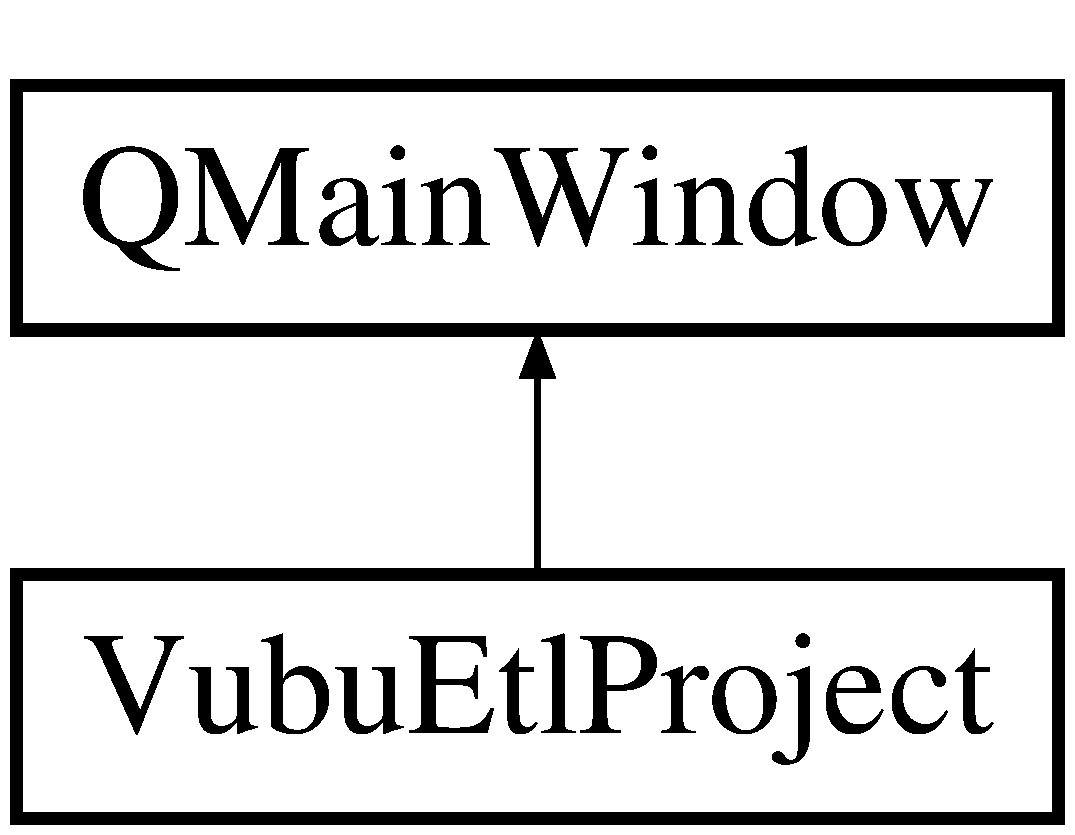
\includegraphics[height=2.000000cm]{class_vubu_etl_project}
\end{center}
\end{figure}
\subsection*{Public Slots}
\begin{DoxyCompactItemize}
\item 
void \mbox{\hyperlink{class_vubu_etl_project_a0ec762e8da4850d4df4a9cc4ca853bc0}{get\+H\+T\+ML}} (Q\+String)
\item 
void \mbox{\hyperlink{class_vubu_etl_project_a96a0529f088b16f27bb5caf4613be354}{transform\+H\+T\+ML}} ()
\begin{DoxyCompactList}\small\item\em Metoda transformuje z pobranych plikow html informacje podane przez uzytkownika. \end{DoxyCompactList}\item 
void \mbox{\hyperlink{class_vubu_etl_project_af2e129dffbe49b95921927226f7f3660}{radio\+Button}} ()
\begin{DoxyCompactList}\small\item\em Metoda generuje rozwijane combo boxy. \end{DoxyCompactList}\item 
void \mbox{\hyperlink{class_vubu_etl_project_ae737e131ae6ce3de41151ac665e6e0d5}{download\+Function}} ()
\begin{DoxyCompactList}\small\item\em Metoda sprawdza jaki aktualnie chackbox jest wcisniety i odpowiednio przekazuje link do rozpoczecia pobierania. \end{DoxyCompactList}\item 
void \mbox{\hyperlink{class_vubu_etl_project_a3079e407acd405007d64fddf84b6f0e6}{update\+Database}} ()
\begin{DoxyCompactList}\small\item\em Metoda zasila baze danych. \end{DoxyCompactList}\item 
void \mbox{\hyperlink{class_vubu_etl_project_a767b72fe3e958c20bb2aa0e11a702f0f}{clear\+Database}} ()
\begin{DoxyCompactList}\small\item\em Metoda czysci baze danych. \end{DoxyCompactList}\item 
void \mbox{\hyperlink{class_vubu_etl_project_af15be1aa31f4d30e0b8c14495848fe49}{get\+H\+T\+M\+L\+Thread}} ()
\begin{DoxyCompactList}\small\item\em Metoda pobiera wszystkie pliki H\+T\+ML. Jest ona uruchamiana w watku. \end{DoxyCompactList}\item 
void \mbox{\hyperlink{class_vubu_etl_project_a2f4f3c71af6c416ba1e3fa90adb742d1}{button\+E\+TL}} ()
\item 
void \mbox{\hyperlink{class_vubu_etl_project_a302013ec97cffed3af6caf652940c9ef}{Thread\+Button\+E\+TL}} ()
\begin{DoxyCompactList}\small\item\em Metoda tworzy watek do uruchomienia procesu E\+TL. \end{DoxyCompactList}\item 
void \mbox{\hyperlink{class_vubu_etl_project_a9f69fb3747b5ecf72d5578dc3664d9ae}{state\+Process}} ()
\begin{DoxyCompactList}\small\item\em Metoda sprawdza i wyswietla odpowiednie komunikaty. \end{DoxyCompactList}\item 
void \mbox{\hyperlink{class_vubu_etl_project_a14c0aae91d0c6e9d0f7a4c749a6a3ea2}{show\+Database}} ()
\begin{DoxyCompactList}\small\item\em Metoda pobiera dane z bazy a nastepnie wyswietla je w tabeli. \end{DoxyCompactList}\item 
void \mbox{\hyperlink{class_vubu_etl_project_a05c6d827c5dadca5127626c6ed6a4ce2}{save\+C\+SV}} ()
\begin{DoxyCompactList}\small\item\em Metoda zapisuje tabele do pliku C\+SV. \end{DoxyCompactList}\end{DoxyCompactItemize}
\subsection*{Public Member Functions}
\begin{DoxyCompactItemize}
\item 
\mbox{\hyperlink{class_vubu_etl_project_abec4bd15669ef0f9090cd3b30dcee4ed}{Vubu\+Etl\+Project}} (Q\+Widget $\ast$parent=Q\+\_\+\+N\+U\+L\+L\+P\+TR)
\item 
\mbox{\hyperlink{class_vubu_etl_project_acdf754deee05e28e8f35682e5b863aab}{$\sim$\+Vubu\+Etl\+Project}} ()
\item 
Q\+String \mbox{\hyperlink{class_vubu_etl_project_aa98aca375afb86994b80a5b88e113a8d}{get\+Value\+File}} (string, int)
\begin{DoxyCompactList}\small\item\em Metoda zwraca dany wiersz w pliku txt. \end{DoxyCompactList}\end{DoxyCompactItemize}
\subsection*{Public Attributes}
\begin{DoxyCompactItemize}
\item 
Q\+String \mbox{\hyperlink{class_vubu_etl_project_a73b7eaeb25ea6a7fd5bbc9565748aa55}{title}}
\item 
Q\+String \mbox{\hyperlink{class_vubu_etl_project_ac2b42c7c93d507c3eb3bdcbd9a762028}{code}}
\item 
Q\+String \mbox{\hyperlink{class_vubu_etl_project_a28c771912257608794a3fa8e3c746c7c}{series}}
\item 
Q\+String \mbox{\hyperlink{class_vubu_etl_project_ab592731b0c19996de933e6676be00d3b}{old\+Price}}
\item 
Q\+String \mbox{\hyperlink{class_vubu_etl_project_a44e6f33f11dd304409f13c146d380abf}{new\+Price}}
\item 
Q\+String \mbox{\hyperlink{class_vubu_etl_project_a695e4e9ea4711a2af8f183860f56f218}{size}}
\item 
Q\+String \mbox{\hyperlink{class_vubu_etl_project_a052dea4f8c17043b3ed20b5c99d40c67}{category}}
\item 
Q\+String \mbox{\hyperlink{class_vubu_etl_project_ac2b56f3b84065b5212789505d94963b6}{under\+Category}}
\item 
Q\+String \mbox{\hyperlink{class_vubu_etl_project_aa94996b4befea6cddbc19a453f32f3f7}{picture}}
\item 
bool \mbox{\hyperlink{class_vubu_etl_project_a99267cd4310daf64856e62edb071b6da}{state}}
\item 
bool \mbox{\hyperlink{class_vubu_etl_project_aec793730a6d756fee5f78af01aff2611}{state\+Button\+E\+TL}}
\item 
bool \mbox{\hyperlink{class_vubu_etl_project_a1eb004aa2b362180cb32f57866ae0530}{state\+Download}}
\item 
bool \mbox{\hyperlink{class_vubu_etl_project_aab858f15bc40065223d9c9735fd7d700}{state\+Download\+Start}}
\item 
bool \mbox{\hyperlink{class_vubu_etl_project_a92c04377e0c8326b29017c617b69e797}{state\+Transform\+Start}}
\item 
bool \mbox{\hyperlink{class_vubu_etl_project_a956e9ade60ebdbf5f09d543ccbc972fc}{state\+Transform\+End}}
\item 
bool \mbox{\hyperlink{class_vubu_etl_project_ac04f10de0f0e066925de4191621ec9ad}{state\+Transform\+Error}}
\item 
bool \mbox{\hyperlink{class_vubu_etl_project_afd522348204bda9d10d6be7da2a86ce8}{state\+Databaseconnect}}
\item 
bool \mbox{\hyperlink{class_vubu_etl_project_ae0c8c525fb34483e86e9a2077dc3ce18}{state\+Database\+Add}}
\item 
bool \mbox{\hyperlink{class_vubu_etl_project_abe8fccc78e282db2ad37ca505d5e5ab1}{state\+Database\+Error}}
\item 
Q\+String \mbox{\hyperlink{class_vubu_etl_project_a098af5530f5fec86634d06cd704b394b}{vubu\+Link}}
\end{DoxyCompactItemize}
\subsection*{Private Member Functions}
\begin{DoxyCompactItemize}
\item 
void \mbox{\hyperlink{class_vubu_etl_project_a64379c0dc064b7b4ca57ff2c627b5cf8}{delete\+Directory}} (string nazwa)
\item 
void \mbox{\hyperlink{class_vubu_etl_project_a1a73781c59eb8b9f5b0c9ed43055adf0}{create\+Directory}} (string nazwa)
\item 
bool \mbox{\hyperlink{class_vubu_etl_project_a61d213ee394551e86a1626a86f8e9aaf}{is\+File}} (Q\+String nazwa)
\item 
void \mbox{\hyperlink{class_vubu_etl_project_a3d68f35327d2d00dc5369312b85364dc}{create\+Table}} (bool)
\begin{DoxyCompactList}\small\item\em Metoda uzupelnia tabele danymi pobranymi z plikow. \end{DoxyCompactList}\end{DoxyCompactItemize}
\subsection*{Private Attributes}
\begin{DoxyCompactItemize}
\item 
string \mbox{\hyperlink{class_vubu_etl_project_a0d4047ff91f3134c7eb7addff54373a5}{wszystkie\+Linki}}
\item 
Ui\+::\+Vubu\+Etl\+Project\+Class \mbox{\hyperlink{class_vubu_etl_project_a8d6acef60edcea1cf1851938baf0955f}{ui}}
\item 
Q\+Timer $\ast$ \mbox{\hyperlink{class_vubu_etl_project_a025e354edb9c556e4aad7e6774b21fd0}{timer}}
\end{DoxyCompactItemize}


\subsection{Constructor \& Destructor Documentation}
\mbox{\Hypertarget{class_vubu_etl_project_abec4bd15669ef0f9090cd3b30dcee4ed}\label{class_vubu_etl_project_abec4bd15669ef0f9090cd3b30dcee4ed}} 
\index{Vubu\+Etl\+Project@{Vubu\+Etl\+Project}!Vubu\+Etl\+Project@{Vubu\+Etl\+Project}}
\index{Vubu\+Etl\+Project@{Vubu\+Etl\+Project}!Vubu\+Etl\+Project@{Vubu\+Etl\+Project}}
\subsubsection{\texorpdfstring{Vubu\+Etl\+Project()}{VubuEtlProject()}}
{\footnotesize\ttfamily Vubu\+Etl\+Project\+::\+Vubu\+Etl\+Project (\begin{DoxyParamCaption}\item[{Q\+Widget $\ast$}]{parent = {\ttfamily Q\+\_\+NULLPTR} }\end{DoxyParamCaption})}

\mbox{\Hypertarget{class_vubu_etl_project_acdf754deee05e28e8f35682e5b863aab}\label{class_vubu_etl_project_acdf754deee05e28e8f35682e5b863aab}} 
\index{Vubu\+Etl\+Project@{Vubu\+Etl\+Project}!````~Vubu\+Etl\+Project@{$\sim$\+Vubu\+Etl\+Project}}
\index{````~Vubu\+Etl\+Project@{$\sim$\+Vubu\+Etl\+Project}!Vubu\+Etl\+Project@{Vubu\+Etl\+Project}}
\subsubsection{\texorpdfstring{$\sim$\+Vubu\+Etl\+Project()}{~VubuEtlProject()}}
{\footnotesize\ttfamily Vubu\+Etl\+Project\+::$\sim$\+Vubu\+Etl\+Project (\begin{DoxyParamCaption}{ }\end{DoxyParamCaption})}



\subsection{Member Function Documentation}
\mbox{\Hypertarget{class_vubu_etl_project_a2f4f3c71af6c416ba1e3fa90adb742d1}\label{class_vubu_etl_project_a2f4f3c71af6c416ba1e3fa90adb742d1}} 
\index{Vubu\+Etl\+Project@{Vubu\+Etl\+Project}!button\+E\+TL@{button\+E\+TL}}
\index{button\+E\+TL@{button\+E\+TL}!Vubu\+Etl\+Project@{Vubu\+Etl\+Project}}
\subsubsection{\texorpdfstring{button\+E\+TL}{buttonETL}}
{\footnotesize\ttfamily void Vubu\+Etl\+Project\+::button\+E\+TL (\begin{DoxyParamCaption}{ }\end{DoxyParamCaption})\hspace{0.3cm}{\ttfamily [slot]}}

Metoda jest wywolywana poprzez wcisniecie przycisku E\+TL Metoda ma za zadanie wykonac caly proces E\+TL \mbox{\Hypertarget{class_vubu_etl_project_a767b72fe3e958c20bb2aa0e11a702f0f}\label{class_vubu_etl_project_a767b72fe3e958c20bb2aa0e11a702f0f}} 
\index{Vubu\+Etl\+Project@{Vubu\+Etl\+Project}!clear\+Database@{clear\+Database}}
\index{clear\+Database@{clear\+Database}!Vubu\+Etl\+Project@{Vubu\+Etl\+Project}}
\subsubsection{\texorpdfstring{clear\+Database}{clearDatabase}}
{\footnotesize\ttfamily void Vubu\+Etl\+Project\+::clear\+Database (\begin{DoxyParamCaption}{ }\end{DoxyParamCaption})\hspace{0.3cm}{\ttfamily [slot]}}



Metoda czysci baze danych. 

\mbox{\Hypertarget{class_vubu_etl_project_a1a73781c59eb8b9f5b0c9ed43055adf0}\label{class_vubu_etl_project_a1a73781c59eb8b9f5b0c9ed43055adf0}} 
\index{Vubu\+Etl\+Project@{Vubu\+Etl\+Project}!create\+Directory@{create\+Directory}}
\index{create\+Directory@{create\+Directory}!Vubu\+Etl\+Project@{Vubu\+Etl\+Project}}
\subsubsection{\texorpdfstring{create\+Directory()}{createDirectory()}}
{\footnotesize\ttfamily void Vubu\+Etl\+Project\+::create\+Directory (\begin{DoxyParamCaption}\item[{string}]{nazwa }\end{DoxyParamCaption})\hspace{0.3cm}{\ttfamily [private]}}

Metoda tworzy folder. Metoda na wejsciu otrzymuje stringa ze sciezka. \mbox{\Hypertarget{class_vubu_etl_project_a3d68f35327d2d00dc5369312b85364dc}\label{class_vubu_etl_project_a3d68f35327d2d00dc5369312b85364dc}} 
\index{Vubu\+Etl\+Project@{Vubu\+Etl\+Project}!create\+Table@{create\+Table}}
\index{create\+Table@{create\+Table}!Vubu\+Etl\+Project@{Vubu\+Etl\+Project}}
\subsubsection{\texorpdfstring{create\+Table()}{createTable()}}
{\footnotesize\ttfamily void Vubu\+Etl\+Project\+::create\+Table (\begin{DoxyParamCaption}\item[{bool}]{warrning }\end{DoxyParamCaption})\hspace{0.3cm}{\ttfamily [private]}}



Metoda uzupelnia tabele danymi pobranymi z plikow. 

\mbox{\Hypertarget{class_vubu_etl_project_a64379c0dc064b7b4ca57ff2c627b5cf8}\label{class_vubu_etl_project_a64379c0dc064b7b4ca57ff2c627b5cf8}} 
\index{Vubu\+Etl\+Project@{Vubu\+Etl\+Project}!delete\+Directory@{delete\+Directory}}
\index{delete\+Directory@{delete\+Directory}!Vubu\+Etl\+Project@{Vubu\+Etl\+Project}}
\subsubsection{\texorpdfstring{delete\+Directory()}{deleteDirectory()}}
{\footnotesize\ttfamily void Vubu\+Etl\+Project\+::delete\+Directory (\begin{DoxyParamCaption}\item[{string}]{nazwa }\end{DoxyParamCaption})\hspace{0.3cm}{\ttfamily [private]}}

Metoda usuwa folder wraz z jej zawartoscia. Metoda na wejsciu otrzymuje stringa ze sciezka. \mbox{\Hypertarget{class_vubu_etl_project_ae737e131ae6ce3de41151ac665e6e0d5}\label{class_vubu_etl_project_ae737e131ae6ce3de41151ac665e6e0d5}} 
\index{Vubu\+Etl\+Project@{Vubu\+Etl\+Project}!download\+Function@{download\+Function}}
\index{download\+Function@{download\+Function}!Vubu\+Etl\+Project@{Vubu\+Etl\+Project}}
\subsubsection{\texorpdfstring{download\+Function}{downloadFunction}}
{\footnotesize\ttfamily void Vubu\+Etl\+Project\+::download\+Function (\begin{DoxyParamCaption}{ }\end{DoxyParamCaption})\hspace{0.3cm}{\ttfamily [slot]}}



Metoda sprawdza jaki aktualnie chackbox jest wcisniety i odpowiednio przekazuje link do rozpoczecia pobierania. 

\mbox{\Hypertarget{class_vubu_etl_project_a0ec762e8da4850d4df4a9cc4ca853bc0}\label{class_vubu_etl_project_a0ec762e8da4850d4df4a9cc4ca853bc0}} 
\index{Vubu\+Etl\+Project@{Vubu\+Etl\+Project}!get\+H\+T\+ML@{get\+H\+T\+ML}}
\index{get\+H\+T\+ML@{get\+H\+T\+ML}!Vubu\+Etl\+Project@{Vubu\+Etl\+Project}}
\subsubsection{\texorpdfstring{get\+H\+T\+ML}{getHTML}}
{\footnotesize\ttfamily void Vubu\+Etl\+Project\+::get\+H\+T\+ML (\begin{DoxyParamCaption}\item[{Q\+String}]{link }\end{DoxyParamCaption})\hspace{0.3cm}{\ttfamily [slot]}}

Metoda aktywuje przycisk do pobierania danych (pliki H\+T\+ML) Na wejsciu otrzymuje link z ktorego ma pobrac dane produkty. \mbox{\Hypertarget{class_vubu_etl_project_af15be1aa31f4d30e0b8c14495848fe49}\label{class_vubu_etl_project_af15be1aa31f4d30e0b8c14495848fe49}} 
\index{Vubu\+Etl\+Project@{Vubu\+Etl\+Project}!get\+H\+T\+M\+L\+Thread@{get\+H\+T\+M\+L\+Thread}}
\index{get\+H\+T\+M\+L\+Thread@{get\+H\+T\+M\+L\+Thread}!Vubu\+Etl\+Project@{Vubu\+Etl\+Project}}
\subsubsection{\texorpdfstring{get\+H\+T\+M\+L\+Thread}{getHTMLThread}}
{\footnotesize\ttfamily void Vubu\+Etl\+Project\+::get\+H\+T\+M\+L\+Thread (\begin{DoxyParamCaption}{ }\end{DoxyParamCaption})\hspace{0.3cm}{\ttfamily [slot]}}



Metoda pobiera wszystkie pliki H\+T\+ML. Jest ona uruchamiana w watku. 

\mbox{\Hypertarget{class_vubu_etl_project_aa98aca375afb86994b80a5b88e113a8d}\label{class_vubu_etl_project_aa98aca375afb86994b80a5b88e113a8d}} 
\index{Vubu\+Etl\+Project@{Vubu\+Etl\+Project}!get\+Value\+File@{get\+Value\+File}}
\index{get\+Value\+File@{get\+Value\+File}!Vubu\+Etl\+Project@{Vubu\+Etl\+Project}}
\subsubsection{\texorpdfstring{get\+Value\+File()}{getValueFile()}}
{\footnotesize\ttfamily Q\+String Vubu\+Etl\+Project\+::get\+Value\+File (\begin{DoxyParamCaption}\item[{string}]{name,  }\item[{int}]{row }\end{DoxyParamCaption})}



Metoda zwraca dany wiersz w pliku txt. 

\mbox{\Hypertarget{class_vubu_etl_project_a61d213ee394551e86a1626a86f8e9aaf}\label{class_vubu_etl_project_a61d213ee394551e86a1626a86f8e9aaf}} 
\index{Vubu\+Etl\+Project@{Vubu\+Etl\+Project}!is\+File@{is\+File}}
\index{is\+File@{is\+File}!Vubu\+Etl\+Project@{Vubu\+Etl\+Project}}
\subsubsection{\texorpdfstring{is\+File()}{isFile()}}
{\footnotesize\ttfamily bool Vubu\+Etl\+Project\+::is\+File (\begin{DoxyParamCaption}\item[{Q\+String}]{nazwa }\end{DoxyParamCaption})\hspace{0.3cm}{\ttfamily [private]}}

Metoda sprawdza czy dany plik istnieje. Metoda na wejsciu otrzymuje stringa ze sciezka. \mbox{\Hypertarget{class_vubu_etl_project_af2e129dffbe49b95921927226f7f3660}\label{class_vubu_etl_project_af2e129dffbe49b95921927226f7f3660}} 
\index{Vubu\+Etl\+Project@{Vubu\+Etl\+Project}!radio\+Button@{radio\+Button}}
\index{radio\+Button@{radio\+Button}!Vubu\+Etl\+Project@{Vubu\+Etl\+Project}}
\subsubsection{\texorpdfstring{radio\+Button}{radioButton}}
{\footnotesize\ttfamily void Vubu\+Etl\+Project\+::radio\+Button (\begin{DoxyParamCaption}{ }\end{DoxyParamCaption})\hspace{0.3cm}{\ttfamily [slot]}}



Metoda generuje rozwijane combo boxy. 

\mbox{\Hypertarget{class_vubu_etl_project_a05c6d827c5dadca5127626c6ed6a4ce2}\label{class_vubu_etl_project_a05c6d827c5dadca5127626c6ed6a4ce2}} 
\index{Vubu\+Etl\+Project@{Vubu\+Etl\+Project}!save\+C\+SV@{save\+C\+SV}}
\index{save\+C\+SV@{save\+C\+SV}!Vubu\+Etl\+Project@{Vubu\+Etl\+Project}}
\subsubsection{\texorpdfstring{save\+C\+SV}{saveCSV}}
{\footnotesize\ttfamily void Vubu\+Etl\+Project\+::save\+C\+SV (\begin{DoxyParamCaption}{ }\end{DoxyParamCaption})\hspace{0.3cm}{\ttfamily [slot]}}



Metoda zapisuje tabele do pliku C\+SV. 

\mbox{\Hypertarget{class_vubu_etl_project_a14c0aae91d0c6e9d0f7a4c749a6a3ea2}\label{class_vubu_etl_project_a14c0aae91d0c6e9d0f7a4c749a6a3ea2}} 
\index{Vubu\+Etl\+Project@{Vubu\+Etl\+Project}!show\+Database@{show\+Database}}
\index{show\+Database@{show\+Database}!Vubu\+Etl\+Project@{Vubu\+Etl\+Project}}
\subsubsection{\texorpdfstring{show\+Database}{showDatabase}}
{\footnotesize\ttfamily void Vubu\+Etl\+Project\+::show\+Database (\begin{DoxyParamCaption}{ }\end{DoxyParamCaption})\hspace{0.3cm}{\ttfamily [slot]}}



Metoda pobiera dane z bazy a nastepnie wyswietla je w tabeli. 

\mbox{\Hypertarget{class_vubu_etl_project_a9f69fb3747b5ecf72d5578dc3664d9ae}\label{class_vubu_etl_project_a9f69fb3747b5ecf72d5578dc3664d9ae}} 
\index{Vubu\+Etl\+Project@{Vubu\+Etl\+Project}!state\+Process@{state\+Process}}
\index{state\+Process@{state\+Process}!Vubu\+Etl\+Project@{Vubu\+Etl\+Project}}
\subsubsection{\texorpdfstring{state\+Process}{stateProcess}}
{\footnotesize\ttfamily void Vubu\+Etl\+Project\+::state\+Process (\begin{DoxyParamCaption}{ }\end{DoxyParamCaption})\hspace{0.3cm}{\ttfamily [slot]}}



Metoda sprawdza i wyswietla odpowiednie komunikaty. 

\mbox{\Hypertarget{class_vubu_etl_project_a302013ec97cffed3af6caf652940c9ef}\label{class_vubu_etl_project_a302013ec97cffed3af6caf652940c9ef}} 
\index{Vubu\+Etl\+Project@{Vubu\+Etl\+Project}!Thread\+Button\+E\+TL@{Thread\+Button\+E\+TL}}
\index{Thread\+Button\+E\+TL@{Thread\+Button\+E\+TL}!Vubu\+Etl\+Project@{Vubu\+Etl\+Project}}
\subsubsection{\texorpdfstring{Thread\+Button\+E\+TL}{ThreadButtonETL}}
{\footnotesize\ttfamily void Vubu\+Etl\+Project\+::\+Thread\+Button\+E\+TL (\begin{DoxyParamCaption}{ }\end{DoxyParamCaption})\hspace{0.3cm}{\ttfamily [slot]}}



Metoda tworzy watek do uruchomienia procesu E\+TL. 

\mbox{\Hypertarget{class_vubu_etl_project_a96a0529f088b16f27bb5caf4613be354}\label{class_vubu_etl_project_a96a0529f088b16f27bb5caf4613be354}} 
\index{Vubu\+Etl\+Project@{Vubu\+Etl\+Project}!transform\+H\+T\+ML@{transform\+H\+T\+ML}}
\index{transform\+H\+T\+ML@{transform\+H\+T\+ML}!Vubu\+Etl\+Project@{Vubu\+Etl\+Project}}
\subsubsection{\texorpdfstring{transform\+H\+T\+ML}{transformHTML}}
{\footnotesize\ttfamily void Vubu\+Etl\+Project\+::transform\+H\+T\+ML (\begin{DoxyParamCaption}{ }\end{DoxyParamCaption})\hspace{0.3cm}{\ttfamily [slot]}}



Metoda transformuje z pobranych plikow html informacje podane przez uzytkownika. 

\mbox{\Hypertarget{class_vubu_etl_project_a3079e407acd405007d64fddf84b6f0e6}\label{class_vubu_etl_project_a3079e407acd405007d64fddf84b6f0e6}} 
\index{Vubu\+Etl\+Project@{Vubu\+Etl\+Project}!update\+Database@{update\+Database}}
\index{update\+Database@{update\+Database}!Vubu\+Etl\+Project@{Vubu\+Etl\+Project}}
\subsubsection{\texorpdfstring{update\+Database}{updateDatabase}}
{\footnotesize\ttfamily void Vubu\+Etl\+Project\+::update\+Database (\begin{DoxyParamCaption}{ }\end{DoxyParamCaption})\hspace{0.3cm}{\ttfamily [slot]}}



Metoda zasila baze danych. 



\subsection{Member Data Documentation}
\mbox{\Hypertarget{class_vubu_etl_project_a052dea4f8c17043b3ed20b5c99d40c67}\label{class_vubu_etl_project_a052dea4f8c17043b3ed20b5c99d40c67}} 
\index{Vubu\+Etl\+Project@{Vubu\+Etl\+Project}!category@{category}}
\index{category@{category}!Vubu\+Etl\+Project@{Vubu\+Etl\+Project}}
\subsubsection{\texorpdfstring{category}{category}}
{\footnotesize\ttfamily Q\+String Vubu\+Etl\+Project\+::category}

\mbox{\Hypertarget{class_vubu_etl_project_ac2b42c7c93d507c3eb3bdcbd9a762028}\label{class_vubu_etl_project_ac2b42c7c93d507c3eb3bdcbd9a762028}} 
\index{Vubu\+Etl\+Project@{Vubu\+Etl\+Project}!code@{code}}
\index{code@{code}!Vubu\+Etl\+Project@{Vubu\+Etl\+Project}}
\subsubsection{\texorpdfstring{code}{code}}
{\footnotesize\ttfamily Q\+String Vubu\+Etl\+Project\+::code}

\mbox{\Hypertarget{class_vubu_etl_project_a44e6f33f11dd304409f13c146d380abf}\label{class_vubu_etl_project_a44e6f33f11dd304409f13c146d380abf}} 
\index{Vubu\+Etl\+Project@{Vubu\+Etl\+Project}!new\+Price@{new\+Price}}
\index{new\+Price@{new\+Price}!Vubu\+Etl\+Project@{Vubu\+Etl\+Project}}
\subsubsection{\texorpdfstring{new\+Price}{newPrice}}
{\footnotesize\ttfamily Q\+String Vubu\+Etl\+Project\+::new\+Price}

\mbox{\Hypertarget{class_vubu_etl_project_ab592731b0c19996de933e6676be00d3b}\label{class_vubu_etl_project_ab592731b0c19996de933e6676be00d3b}} 
\index{Vubu\+Etl\+Project@{Vubu\+Etl\+Project}!old\+Price@{old\+Price}}
\index{old\+Price@{old\+Price}!Vubu\+Etl\+Project@{Vubu\+Etl\+Project}}
\subsubsection{\texorpdfstring{old\+Price}{oldPrice}}
{\footnotesize\ttfamily Q\+String Vubu\+Etl\+Project\+::old\+Price}

\mbox{\Hypertarget{class_vubu_etl_project_aa94996b4befea6cddbc19a453f32f3f7}\label{class_vubu_etl_project_aa94996b4befea6cddbc19a453f32f3f7}} 
\index{Vubu\+Etl\+Project@{Vubu\+Etl\+Project}!picture@{picture}}
\index{picture@{picture}!Vubu\+Etl\+Project@{Vubu\+Etl\+Project}}
\subsubsection{\texorpdfstring{picture}{picture}}
{\footnotesize\ttfamily Q\+String Vubu\+Etl\+Project\+::picture}

\mbox{\Hypertarget{class_vubu_etl_project_a28c771912257608794a3fa8e3c746c7c}\label{class_vubu_etl_project_a28c771912257608794a3fa8e3c746c7c}} 
\index{Vubu\+Etl\+Project@{Vubu\+Etl\+Project}!series@{series}}
\index{series@{series}!Vubu\+Etl\+Project@{Vubu\+Etl\+Project}}
\subsubsection{\texorpdfstring{series}{series}}
{\footnotesize\ttfamily Q\+String Vubu\+Etl\+Project\+::series}

\mbox{\Hypertarget{class_vubu_etl_project_a695e4e9ea4711a2af8f183860f56f218}\label{class_vubu_etl_project_a695e4e9ea4711a2af8f183860f56f218}} 
\index{Vubu\+Etl\+Project@{Vubu\+Etl\+Project}!size@{size}}
\index{size@{size}!Vubu\+Etl\+Project@{Vubu\+Etl\+Project}}
\subsubsection{\texorpdfstring{size}{size}}
{\footnotesize\ttfamily Q\+String Vubu\+Etl\+Project\+::size}

\mbox{\Hypertarget{class_vubu_etl_project_a99267cd4310daf64856e62edb071b6da}\label{class_vubu_etl_project_a99267cd4310daf64856e62edb071b6da}} 
\index{Vubu\+Etl\+Project@{Vubu\+Etl\+Project}!state@{state}}
\index{state@{state}!Vubu\+Etl\+Project@{Vubu\+Etl\+Project}}
\subsubsection{\texorpdfstring{state}{state}}
{\footnotesize\ttfamily bool Vubu\+Etl\+Project\+::state}

\mbox{\Hypertarget{class_vubu_etl_project_aec793730a6d756fee5f78af01aff2611}\label{class_vubu_etl_project_aec793730a6d756fee5f78af01aff2611}} 
\index{Vubu\+Etl\+Project@{Vubu\+Etl\+Project}!state\+Button\+E\+TL@{state\+Button\+E\+TL}}
\index{state\+Button\+E\+TL@{state\+Button\+E\+TL}!Vubu\+Etl\+Project@{Vubu\+Etl\+Project}}
\subsubsection{\texorpdfstring{state\+Button\+E\+TL}{stateButtonETL}}
{\footnotesize\ttfamily bool Vubu\+Etl\+Project\+::state\+Button\+E\+TL}

\mbox{\Hypertarget{class_vubu_etl_project_ae0c8c525fb34483e86e9a2077dc3ce18}\label{class_vubu_etl_project_ae0c8c525fb34483e86e9a2077dc3ce18}} 
\index{Vubu\+Etl\+Project@{Vubu\+Etl\+Project}!state\+Database\+Add@{state\+Database\+Add}}
\index{state\+Database\+Add@{state\+Database\+Add}!Vubu\+Etl\+Project@{Vubu\+Etl\+Project}}
\subsubsection{\texorpdfstring{state\+Database\+Add}{stateDatabaseAdd}}
{\footnotesize\ttfamily bool Vubu\+Etl\+Project\+::state\+Database\+Add}

\mbox{\Hypertarget{class_vubu_etl_project_afd522348204bda9d10d6be7da2a86ce8}\label{class_vubu_etl_project_afd522348204bda9d10d6be7da2a86ce8}} 
\index{Vubu\+Etl\+Project@{Vubu\+Etl\+Project}!state\+Databaseconnect@{state\+Databaseconnect}}
\index{state\+Databaseconnect@{state\+Databaseconnect}!Vubu\+Etl\+Project@{Vubu\+Etl\+Project}}
\subsubsection{\texorpdfstring{state\+Databaseconnect}{stateDatabaseconnect}}
{\footnotesize\ttfamily bool Vubu\+Etl\+Project\+::state\+Databaseconnect}

\mbox{\Hypertarget{class_vubu_etl_project_abe8fccc78e282db2ad37ca505d5e5ab1}\label{class_vubu_etl_project_abe8fccc78e282db2ad37ca505d5e5ab1}} 
\index{Vubu\+Etl\+Project@{Vubu\+Etl\+Project}!state\+Database\+Error@{state\+Database\+Error}}
\index{state\+Database\+Error@{state\+Database\+Error}!Vubu\+Etl\+Project@{Vubu\+Etl\+Project}}
\subsubsection{\texorpdfstring{state\+Database\+Error}{stateDatabaseError}}
{\footnotesize\ttfamily bool Vubu\+Etl\+Project\+::state\+Database\+Error}

\mbox{\Hypertarget{class_vubu_etl_project_a1eb004aa2b362180cb32f57866ae0530}\label{class_vubu_etl_project_a1eb004aa2b362180cb32f57866ae0530}} 
\index{Vubu\+Etl\+Project@{Vubu\+Etl\+Project}!state\+Download@{state\+Download}}
\index{state\+Download@{state\+Download}!Vubu\+Etl\+Project@{Vubu\+Etl\+Project}}
\subsubsection{\texorpdfstring{state\+Download}{stateDownload}}
{\footnotesize\ttfamily bool Vubu\+Etl\+Project\+::state\+Download}

\mbox{\Hypertarget{class_vubu_etl_project_aab858f15bc40065223d9c9735fd7d700}\label{class_vubu_etl_project_aab858f15bc40065223d9c9735fd7d700}} 
\index{Vubu\+Etl\+Project@{Vubu\+Etl\+Project}!state\+Download\+Start@{state\+Download\+Start}}
\index{state\+Download\+Start@{state\+Download\+Start}!Vubu\+Etl\+Project@{Vubu\+Etl\+Project}}
\subsubsection{\texorpdfstring{state\+Download\+Start}{stateDownloadStart}}
{\footnotesize\ttfamily bool Vubu\+Etl\+Project\+::state\+Download\+Start}

\mbox{\Hypertarget{class_vubu_etl_project_a956e9ade60ebdbf5f09d543ccbc972fc}\label{class_vubu_etl_project_a956e9ade60ebdbf5f09d543ccbc972fc}} 
\index{Vubu\+Etl\+Project@{Vubu\+Etl\+Project}!state\+Transform\+End@{state\+Transform\+End}}
\index{state\+Transform\+End@{state\+Transform\+End}!Vubu\+Etl\+Project@{Vubu\+Etl\+Project}}
\subsubsection{\texorpdfstring{state\+Transform\+End}{stateTransformEnd}}
{\footnotesize\ttfamily bool Vubu\+Etl\+Project\+::state\+Transform\+End}

\mbox{\Hypertarget{class_vubu_etl_project_ac04f10de0f0e066925de4191621ec9ad}\label{class_vubu_etl_project_ac04f10de0f0e066925de4191621ec9ad}} 
\index{Vubu\+Etl\+Project@{Vubu\+Etl\+Project}!state\+Transform\+Error@{state\+Transform\+Error}}
\index{state\+Transform\+Error@{state\+Transform\+Error}!Vubu\+Etl\+Project@{Vubu\+Etl\+Project}}
\subsubsection{\texorpdfstring{state\+Transform\+Error}{stateTransformError}}
{\footnotesize\ttfamily bool Vubu\+Etl\+Project\+::state\+Transform\+Error}

\mbox{\Hypertarget{class_vubu_etl_project_a92c04377e0c8326b29017c617b69e797}\label{class_vubu_etl_project_a92c04377e0c8326b29017c617b69e797}} 
\index{Vubu\+Etl\+Project@{Vubu\+Etl\+Project}!state\+Transform\+Start@{state\+Transform\+Start}}
\index{state\+Transform\+Start@{state\+Transform\+Start}!Vubu\+Etl\+Project@{Vubu\+Etl\+Project}}
\subsubsection{\texorpdfstring{state\+Transform\+Start}{stateTransformStart}}
{\footnotesize\ttfamily bool Vubu\+Etl\+Project\+::state\+Transform\+Start}

\mbox{\Hypertarget{class_vubu_etl_project_a025e354edb9c556e4aad7e6774b21fd0}\label{class_vubu_etl_project_a025e354edb9c556e4aad7e6774b21fd0}} 
\index{Vubu\+Etl\+Project@{Vubu\+Etl\+Project}!timer@{timer}}
\index{timer@{timer}!Vubu\+Etl\+Project@{Vubu\+Etl\+Project}}
\subsubsection{\texorpdfstring{timer}{timer}}
{\footnotesize\ttfamily Q\+Timer$\ast$ Vubu\+Etl\+Project\+::timer\hspace{0.3cm}{\ttfamily [private]}}

\mbox{\Hypertarget{class_vubu_etl_project_a73b7eaeb25ea6a7fd5bbc9565748aa55}\label{class_vubu_etl_project_a73b7eaeb25ea6a7fd5bbc9565748aa55}} 
\index{Vubu\+Etl\+Project@{Vubu\+Etl\+Project}!title@{title}}
\index{title@{title}!Vubu\+Etl\+Project@{Vubu\+Etl\+Project}}
\subsubsection{\texorpdfstring{title}{title}}
{\footnotesize\ttfamily Q\+String Vubu\+Etl\+Project\+::title}

\mbox{\Hypertarget{class_vubu_etl_project_a8d6acef60edcea1cf1851938baf0955f}\label{class_vubu_etl_project_a8d6acef60edcea1cf1851938baf0955f}} 
\index{Vubu\+Etl\+Project@{Vubu\+Etl\+Project}!ui@{ui}}
\index{ui@{ui}!Vubu\+Etl\+Project@{Vubu\+Etl\+Project}}
\subsubsection{\texorpdfstring{ui}{ui}}
{\footnotesize\ttfamily Ui\+::\+Vubu\+Etl\+Project\+Class Vubu\+Etl\+Project\+::ui\hspace{0.3cm}{\ttfamily [private]}}

\mbox{\Hypertarget{class_vubu_etl_project_ac2b56f3b84065b5212789505d94963b6}\label{class_vubu_etl_project_ac2b56f3b84065b5212789505d94963b6}} 
\index{Vubu\+Etl\+Project@{Vubu\+Etl\+Project}!under\+Category@{under\+Category}}
\index{under\+Category@{under\+Category}!Vubu\+Etl\+Project@{Vubu\+Etl\+Project}}
\subsubsection{\texorpdfstring{under\+Category}{underCategory}}
{\footnotesize\ttfamily Q\+String Vubu\+Etl\+Project\+::under\+Category}

\mbox{\Hypertarget{class_vubu_etl_project_a098af5530f5fec86634d06cd704b394b}\label{class_vubu_etl_project_a098af5530f5fec86634d06cd704b394b}} 
\index{Vubu\+Etl\+Project@{Vubu\+Etl\+Project}!vubu\+Link@{vubu\+Link}}
\index{vubu\+Link@{vubu\+Link}!Vubu\+Etl\+Project@{Vubu\+Etl\+Project}}
\subsubsection{\texorpdfstring{vubu\+Link}{vubuLink}}
{\footnotesize\ttfamily Q\+String Vubu\+Etl\+Project\+::vubu\+Link}

\mbox{\Hypertarget{class_vubu_etl_project_a0d4047ff91f3134c7eb7addff54373a5}\label{class_vubu_etl_project_a0d4047ff91f3134c7eb7addff54373a5}} 
\index{Vubu\+Etl\+Project@{Vubu\+Etl\+Project}!wszystkie\+Linki@{wszystkie\+Linki}}
\index{wszystkie\+Linki@{wszystkie\+Linki}!Vubu\+Etl\+Project@{Vubu\+Etl\+Project}}
\subsubsection{\texorpdfstring{wszystkie\+Linki}{wszystkieLinki}}
{\footnotesize\ttfamily string Vubu\+Etl\+Project\+::wszystkie\+Linki\hspace{0.3cm}{\ttfamily [private]}}



The documentation for this class was generated from the following files\+:\begin{DoxyCompactItemize}
\item 
\mbox{\hyperlink{_vubu_etl_project_8h}{Vubu\+Etl\+Project.\+h}}\item 
\mbox{\hyperlink{_vubu_etl_project_8cpp}{Vubu\+Etl\+Project.\+cpp}}\end{DoxyCompactItemize}

\chapter{File Documentation}
\hypertarget{bd_sql_8cpp}{}\section{bd\+Sql.\+cpp File Reference}
\label{bd_sql_8cpp}\index{bd\+Sql.\+cpp@{bd\+Sql.\+cpp}}
{\ttfamily \#include \char`\"{}bd\+Sql.\+h\char`\"{}}\newline
\subsection*{Variables}
\begin{DoxyCompactItemize}
\item 
sqlite3 $\ast$ \mbox{\hyperlink{bd_sql_8cpp_a4f552f29e4635fa318b9e5d46cd597b3}{dbsql}}
\end{DoxyCompactItemize}


\subsection{Variable Documentation}
\mbox{\Hypertarget{bd_sql_8cpp_a4f552f29e4635fa318b9e5d46cd597b3}\label{bd_sql_8cpp_a4f552f29e4635fa318b9e5d46cd597b3}} 
\index{bd\+Sql.\+cpp@{bd\+Sql.\+cpp}!dbsql@{dbsql}}
\index{dbsql@{dbsql}!bd\+Sql.\+cpp@{bd\+Sql.\+cpp}}
\subsubsection{\texorpdfstring{dbsql}{dbsql}}
{\footnotesize\ttfamily sqlite3$\ast$ dbsql}


\hypertarget{bd_sql_8h}{}\section{bd\+Sql.\+h File Reference}
\label{bd_sql_8h}\index{bd\+Sql.\+h@{bd\+Sql.\+h}}
{\ttfamily \#include \char`\"{}Vubu\+Etl\+Project.\+h\char`\"{}}\newline
\subsection*{Classes}
\begin{DoxyCompactItemize}
\item 
class \mbox{\hyperlink{classbd_sql}{bd\+Sql}}
\end{DoxyCompactItemize}

\hypertarget{download_product_8cpp}{}\section{download\+Product.\+cpp File Reference}
\label{download_product_8cpp}\index{download\+Product.\+cpp@{download\+Product.\+cpp}}
{\ttfamily \#include \char`\"{}download\+Product.\+h\char`\"{}}\newline

\hypertarget{download_product_8h}{}\section{download\+Product.\+h File Reference}
\label{download_product_8h}\index{download\+Product.\+h@{download\+Product.\+h}}
{\ttfamily \#include \char`\"{}Vubu\+Etl\+Project.\+h\char`\"{}}\newline
\subsection*{Classes}
\begin{DoxyCompactItemize}
\item 
class \mbox{\hyperlink{classdownload_product}{download\+Product}}
\end{DoxyCompactItemize}

\hypertarget{main_8cpp}{}\section{main.\+cpp File Reference}
\label{main_8cpp}\index{main.\+cpp@{main.\+cpp}}
{\ttfamily \#include \char`\"{}Vubu\+Etl\+Project.\+h\char`\"{}}\newline
{\ttfamily \#include $<$Qt\+Widgets/\+Q\+Application$>$}\newline
\subsection*{Functions}
\begin{DoxyCompactItemize}
\item 
int \mbox{\hyperlink{main_8cpp_a0ddf1224851353fc92bfbff6f499fa97}{main}} (int argc, char $\ast$argv\mbox{[}$\,$\mbox{]})
\end{DoxyCompactItemize}


\subsection{Function Documentation}
\mbox{\Hypertarget{main_8cpp_a0ddf1224851353fc92bfbff6f499fa97}\label{main_8cpp_a0ddf1224851353fc92bfbff6f499fa97}} 
\index{main.\+cpp@{main.\+cpp}!main@{main}}
\index{main@{main}!main.\+cpp@{main.\+cpp}}
\subsubsection{\texorpdfstring{main()}{main()}}
{\footnotesize\ttfamily int main (\begin{DoxyParamCaption}\item[{int}]{argc,  }\item[{char $\ast$}]{argv\mbox{[}$\,$\mbox{]} }\end{DoxyParamCaption})}


\hypertarget{table_8cpp}{}\section{table.\+cpp File Reference}
\label{table_8cpp}\index{table.\+cpp@{table.\+cpp}}
{\ttfamily \#include \char`\"{}table.\+h\char`\"{}}\newline

\hypertarget{table_8h}{}\section{table.\+h File Reference}
\label{table_8h}\index{table.\+h@{table.\+h}}
{\ttfamily \#include \char`\"{}Vubu\+Etl\+Project.\+h\char`\"{}}\newline
{\ttfamily \#include $<$Q\+File\+Dialog$>$}\newline
\subsection*{Classes}
\begin{DoxyCompactItemize}
\item 
class \mbox{\hyperlink{classtable}{table}}
\end{DoxyCompactItemize}

\hypertarget{transform_file_8cpp}{}\section{transform\+File.\+cpp File Reference}
\label{transform_file_8cpp}\index{transform\+File.\+cpp@{transform\+File.\+cpp}}
{\ttfamily \#include \char`\"{}transform\+File.\+h\char`\"{}}\newline
{\ttfamily \#include $<$locale$>$}\newline
{\ttfamily \#include $<$codecvt$>$}\newline

\hypertarget{transform_file_8h}{}\section{transform\+File.\+h File Reference}
\label{transform_file_8h}\index{transform\+File.\+h@{transform\+File.\+h}}
{\ttfamily \#include \char`\"{}Vubu\+Etl\+Project.\+h\char`\"{}}\newline
\subsection*{Classes}
\begin{DoxyCompactItemize}
\item 
class \mbox{\hyperlink{classtransform_file}{transform\+File}}
\end{DoxyCompactItemize}

\hypertarget{_vubu_etl_project_8cpp}{}\section{Vubu\+Etl\+Project.\+cpp File Reference}
\label{_vubu_etl_project_8cpp}\index{Vubu\+Etl\+Project.\+cpp@{Vubu\+Etl\+Project.\+cpp}}
{\ttfamily \#include \char`\"{}Vubu\+Etl\+Project.\+h\char`\"{}}\newline
\subsection*{Variables}
\begin{DoxyCompactItemize}
\item 
\mbox{\hyperlink{classdownload_product}{download\+Product}} \mbox{\hyperlink{_vubu_etl_project_8cpp_a3b381dafe3f1caf121614944e1a5841c}{download\+ButtonE}}
\item 
\mbox{\hyperlink{classtransform_file}{transform\+File}} \mbox{\hyperlink{_vubu_etl_project_8cpp_a77394c613d2d19b6c21f16c99b93204a}{transform\+ButtonT}}
\item 
\mbox{\hyperlink{classtable}{table}} \mbox{\hyperlink{_vubu_etl_project_8cpp_a41a512dd062380b2fb72a606624bff6f}{table\+Project}}
\item 
\mbox{\hyperlink{classbd_sql}{bd\+Sql}} \mbox{\hyperlink{_vubu_etl_project_8cpp_a006dfa25d6accfee7ad79add10d1a301}{data\+Base}}
\end{DoxyCompactItemize}


\subsection{Variable Documentation}
\mbox{\Hypertarget{_vubu_etl_project_8cpp_a006dfa25d6accfee7ad79add10d1a301}\label{_vubu_etl_project_8cpp_a006dfa25d6accfee7ad79add10d1a301}} 
\index{Vubu\+Etl\+Project.\+cpp@{Vubu\+Etl\+Project.\+cpp}!data\+Base@{data\+Base}}
\index{data\+Base@{data\+Base}!Vubu\+Etl\+Project.\+cpp@{Vubu\+Etl\+Project.\+cpp}}
\subsubsection{\texorpdfstring{data\+Base}{dataBase}}
{\footnotesize\ttfamily \mbox{\hyperlink{classbd_sql}{bd\+Sql}} data\+Base}

\mbox{\Hypertarget{_vubu_etl_project_8cpp_a3b381dafe3f1caf121614944e1a5841c}\label{_vubu_etl_project_8cpp_a3b381dafe3f1caf121614944e1a5841c}} 
\index{Vubu\+Etl\+Project.\+cpp@{Vubu\+Etl\+Project.\+cpp}!download\+ButtonE@{download\+ButtonE}}
\index{download\+ButtonE@{download\+ButtonE}!Vubu\+Etl\+Project.\+cpp@{Vubu\+Etl\+Project.\+cpp}}
\subsubsection{\texorpdfstring{download\+ButtonE}{downloadButtonE}}
{\footnotesize\ttfamily \mbox{\hyperlink{classdownload_product}{download\+Product}} download\+ButtonE}

\mbox{\Hypertarget{_vubu_etl_project_8cpp_a41a512dd062380b2fb72a606624bff6f}\label{_vubu_etl_project_8cpp_a41a512dd062380b2fb72a606624bff6f}} 
\index{Vubu\+Etl\+Project.\+cpp@{Vubu\+Etl\+Project.\+cpp}!table\+Project@{table\+Project}}
\index{table\+Project@{table\+Project}!Vubu\+Etl\+Project.\+cpp@{Vubu\+Etl\+Project.\+cpp}}
\subsubsection{\texorpdfstring{table\+Project}{tableProject}}
{\footnotesize\ttfamily \mbox{\hyperlink{classtable}{table}} table\+Project}

\mbox{\Hypertarget{_vubu_etl_project_8cpp_a77394c613d2d19b6c21f16c99b93204a}\label{_vubu_etl_project_8cpp_a77394c613d2d19b6c21f16c99b93204a}} 
\index{Vubu\+Etl\+Project.\+cpp@{Vubu\+Etl\+Project.\+cpp}!transform\+ButtonT@{transform\+ButtonT}}
\index{transform\+ButtonT@{transform\+ButtonT}!Vubu\+Etl\+Project.\+cpp@{Vubu\+Etl\+Project.\+cpp}}
\subsubsection{\texorpdfstring{transform\+ButtonT}{transformButtonT}}
{\footnotesize\ttfamily \mbox{\hyperlink{classtransform_file}{transform\+File}} transform\+ButtonT}


\hypertarget{_vubu_etl_project_8h}{}\section{Vubu\+Etl\+Project.\+h File Reference}
\label{_vubu_etl_project_8h}\index{Vubu\+Etl\+Project.\+h@{Vubu\+Etl\+Project.\+h}}
{\ttfamily \#include $<$Qt\+Widgets/\+Q\+Main\+Window$>$}\newline
{\ttfamily \#include $<$Q\+Application$>$}\newline
{\ttfamily \#include $<$Qt\+Gui$>$}\newline
{\ttfamily \#include $<$Qt\+Sql$>$}\newline
{\ttfamily \#include $<$Q\+Sql\+Database$>$}\newline
{\ttfamily \#include $<$Q\+File\+Info$>$}\newline
{\ttfamily \#include $<$Qt\+Xml$>$}\newline
{\ttfamily \#include $<$thread$>$}\newline
{\ttfamily \#include \char`\"{}ui\+\_\+\+Vubu\+Etl\+Project.\+h\char`\"{}}\newline
{\ttfamily \#include \char`\"{}download\+Product.\+h\char`\"{}}\newline
{\ttfamily \#include \char`\"{}transform\+File.\+h\char`\"{}}\newline
{\ttfamily \#include \char`\"{}bd\+Sql.\+h\char`\"{}}\newline
{\ttfamily \#include \char`\"{}table.\+h\char`\"{}}\newline
{\ttfamily \#include $<$iostream$>$}\newline
{\ttfamily \#include $<$conio.\+h$>$}\newline
{\ttfamily \#include $<$urlmon.\+h$>$}\newline
{\ttfamily \#include $<$string$>$}\newline
{\ttfamily \#include $<$fstream$>$}\newline
{\ttfamily \#include $<$winsqlite/winsqlite3.\+h$>$}\newline
\subsection*{Classes}
\begin{DoxyCompactItemize}
\item 
class \mbox{\hyperlink{class_vubu_etl_project}{Vubu\+Etl\+Project}}
\end{DoxyCompactItemize}

%--- End generated contents ---

% Index
\backmatter
\newpage
\phantomsection
\clearemptydoublepage
\addcontentsline{toc}{chapter}{Index}
\printindex

\end{document}
